\documentclass{article}
\usepackage{graphicx}
\usepackage{wrapfig}
\usepackage{subcaption}
\usepackage[margin=1in]{geometry}
\usepackage{amsmath} % or simply amstext
\usepackage{siunitx}
\usepackage{booktabs}
\usepackage[export]{adjustbox}
\newcommand{\angstrom}{\textup{\AA}}
\usepackage{cleveref}
\usepackage{booktabs}
\usepackage{gensymb}
\usepackage{float}
%MRS: paper needs a conclusions section outlined.
%MRS: maybe replace pi with $\pi$,qz with $q_z$, and \angstrom by \angstrom~ (the tilde is an enforced space)
%MRS: also maybe \AA instead of \angstrom?  I can't remember which formats better in text.
%\title{Predicting Transport in Lyotropic Liquid Crystal Membranes with Molecular Dynamics Simulations -- Outline}
%MRS: focus isn't really on transport, but on what the strucures are.
\title{Understanding the nanoscale structure of hexagonal phase lyotropic liquid crystal membranes}
%MRS: I don't know that we need to put MD simulations alone in the title, since we also do a fair amount of comparison to experiment. 
\author{Benjamin J. Coscia \and Douglas L. Gin \and Richard D. Noble \and Joe Yelk \and Matthew Glaser \and Xunda Feng \and Michael R. Shirts} 
\begin{document}
  \bibliographystyle{ieeetr}
  \graphicspath{{./figures/}}
  \maketitle
  \section*{Introduction}
  
  Nanostructured membrane materials have become increasingly popular for 
  aqueous separations applications such as desalination and biorefinement
  because they offer the ability to control membrane architecture at the
  atomic scale allowing the design of solute-specific separation membranes. \cite{humplik_nanostructured_2011}
  \begin{itemize}
    \item Most membrane-based aqueous separations of small molecules can 
    be achieved using reverse osmosis (RO) or nanofiltration (NF) \cite{van_der_bruggen_review_2003}
  \end{itemize}
  
  While RO and NF have seen many advances in the past few decades, they 
  are far from perfect separation technologies.
  \begin{itemize}
    \item \textit{RO membranes}
    \item \textbf{Inconsistent performance} : Current state-of-the-art RO membranes are unstructured with
    tortuous and polydisperse diffusion pathways which leads to 
    inconsistent performance \cite{song_nano_2011}
    \item \textbf{High energy requirements} : Necessarily high feed pressures 
    drive up energy requirements which strains developing regions and
    contributes strongly to CO\textsubscript{2} emissions. \cite{mcginnis_global_2008}
    \item \textbf{Separation based on differences in solubility and diffusivity}:
    Moreover, designing RO membranes to achieve targeted separations of 
    specific solutes is nearly impossible because various solutes dissolve
    into and diffuse through the polymer matrix at different rates. \cite{wijmans_solution-diffusion_1995}
    \item At best, one can exploit these differences to create a functional
    selective barrier.
    \item \textit{NF membranes}
    \item NF was introduced as an intermediate between RO and ultrafiltration,
    having the ability to separate organic matter and salts on the order of 
    one nanometer in size.
    \item Larger and well-defined pores drive down energy requirements while
    still affording separation of solutes as small as ions to some degree \cite{van_der_bruggen_review_2003}
    \item NF is often used as a precursor to reverse osmosis
    \item Unfortunately, NF membranes, like RO, are produced with a pore size 
    distribution which limits their ability to perform precise separations \cite{bowen_modelling_2002}
  \end{itemize}
  
  Nanostructured membranes can bypass many of the performance issues which
  plague traditional NF and RO membranes.
  \begin{itemize}
    \item \textbf{Tune size and functionality of building blocks} to control pore
    size and shape: One can accomplish targeted separations with high 
    selectivity by tuning shape, size and functionality of the molecular
    building blocks which form these materials. % BJC: "these materials" --> "nanostructured membranes", or is that redundant?
    \item As a result, solute rejecting pores can have their sizes tuned
    uniformly, resulting in \textbf{strict size cut-offs}.
    \item Entirely \textbf{different mechanisms} may govern transport in a given
    nanostructured material which can inspire novel separation techniques.
  \end{itemize}
  
  Development of nanostructured materials has been limited by the ability
  to synthesize and scale various fundamentally sound technologies.
  \begin{itemize}
    \item \textbf{Graphene sheets} are atomically thick which results in excellent
    permeability but defects during manufacturing severely impact 
    selectivity. \cite{cohen-tanugi_multilayer_2016}
    \item Molecular dynamics simulations of \textbf{carbon nanotubes} show
    promise \cite{humplik_nanostructured_2011} but synthetic techniques are 
    unable to achieve scalable alignment and pore monodispersity.\cite{hata_water-assisted_2004,maruyama_growth_2005}
    \item \textbf{Zeolites} have sub-nm pores with a narrow pore size 
    distribution and MD simulations exhibit complete rejection of solvated ions, \cite{murad_molecular_1998}
    however, experimental rejection was low and attributed to interstitial
    defects formed during membrane synthesis \cite{li_desalination_2004}
    \item There is a need for a scalable nanostructured membrane
  \end{itemize}
  
  Self assembling lyotropic liquid crystals (LLCs) are a suitable candidate for
  aqueous separation applications. 
  \begin{itemize}
    \item LLCs share the characteristic ability of nanostructured membrane
    materials to create \textbf{highly ordered structures} with the added benefits
    of \textbf{low cost} and synthetic techniques feasible for 
    \textbf{large scale production} \cite{feng_scalable_2014}
    \item Neat liquid crystal monomer forms the thermotropic, Col\textsubscript{h}
    phase. The presence of small amounts of water results in the H\textsubscript{II} 
    phase.
    \item In both cases, monomers assemble into mesophases made of hexagonally
    packed, uniform size, cylinders with hydrophilic groups oriented inward
    towards the pore center and hydrophobic groups facing outward.
    \item H\textsubscript{II} and Col\textsubscript{h} phase systems created by
    the monomer named Na-GA3C11 has been extensively studied experimentally \cite{smith_ordered_1997, %BJC: IUPAC chemical name here?
    zhou_supported_2005,resel_h2-phase_2000,feng_scalable_2014,feng_thin_2016}. 
    \item Until recently, mesophases formed by Na-GA3C11 could not be macroscopically
    aligned, resulting in a low flux membrane, slowing research in the field.
    \item In 2014, Feng et al. showed that the mesophases could be aligned 
    using a magnetic field with subsequent crosslinking to lock the structure
    in place \cite{feng_scalable_2014}
    \item In 2016, Feng et al. showed that the same result could be obtained 
    using a technique termed soft confinement \cite{feng_thin_2016}.
    \item Following this breakthrough, research into LLC membranes has been
    reinvigorated
  \end{itemize}
  
  A molecular level understanding of LLC membrane structure, enabled by molecular
  dynamics simulations, will provide guidelines to reduce the large chemical space
  available to design monomers for creation of separation-specific membranes.
  \begin{itemize}
%     \item LLCs are versatile and controllable with a \textbf{large chemical design
%     space} available for membrane design  %BJC: redundant
    \item  We do not yet understand how to reduce the effective pore size or 
    how to tune the chemical environment in the nanopores for effective water
    desalination or small organic molecule separations.
    \item Rejection studies show that this membrane can not perform separations of
    solutes less than 1.2 nm because the pores are too large \cite{zhou_supported_2005}.
    \item Over the past 20 years, LLC membrane studies have been limited primarily 
    to Na-GA3C11 with some characterization done after minor structural modifications
    \cite{resel_structural_2000}. 
    \item Optimization has been performed through trial and error. The only source of 
    predictive modeling has been macroscopic models which likely do not adequately describe 
    transport at these length scales. % BJC: Reference. I think it is just w.r.t. bicontinuous cubic
    \item It will be challenging to efficiently narrow down the design space in 
    a laboratory setting.
    \item A good molecular model should incorporate a detailed picture of the nanoscopic pore 
    structure which will be crucial to understanding the role of monomer structure in 
    membrane design.
    \item Choice of head group may play a role in the rejection of charged or uncharged solutes.
    \item Choice of counterion may influence the establishment of a Donnan potential 
    affecting the degree to which the membrane can exclude charged species.
    \item Moieties inside the pores may interact with neutral solutes, rejecting
    on the basis of shape and 
    %MRS: size pretty much is hydrodynamic radius
    %size, 
    interactions with specific chemical groups
rather than just hydrodynamic radius.
    %MRS: isn't this next point just a restatement of what was said at the top?
    %BJC: yes, deleted
  \end{itemize}
  
  Our approach to constructing a general model will be based on the development of a
  model of a specific LLC membrane which has ample experimental characterization. %BJC: ample too much?
    \begin{itemize}
    \item We have chosen to focus on assemblies formed by Na-GA3C11
    \item We have also narrowed our scope to the development of 
    a model of the Col\textsubscript{h} phase membrane.
    \item Compared to the H\textsubscript{II} phase, the Col\textsubscript{h}
    phase is a simpler starting point, due to the absence of water, and has
    equivalent experimental structural data.
    \item Despite having structural data, there is still information which 
    experiment cannot definitively answer
    \end{itemize}

%BJC: the following just seems like filler now that I've reorganized
%   A clear picture of the nanoscopic LLC membrane structure, gained by building 
%   a molecular model will provide evidence to answer existing and newly proposed
%   questions.
%     \begin{itemize}
%     \item Despite having structural data, there is still information which 
%     experiment cannot definitively answer
%     \end{itemize}

%MRS: break this down into more hierarchy - there are 11 separate points.  Can they be grouped at all for clearer understanding? elucidate what the aspects are we need a clearer picture. 
%BJC: I moved the logic for choice of monomer to system to model to a separate paragraph (above this). I then moved the other three things I talk about into their own paragraphs to keep the ideas separate (following paragraphs).

%MRS: since the questions we answer in the paper have a lot to do with the structure of the membranes, somewhere relatively early in the paper we need to lay out the facts that 1) these membranes could be really good (I think you do establish this) 2) we really would need to know the structure better to really do useful things with these, and 3) MD is a very helpful way to gain more information about the structure, because of the limited range of experiments we can do with these systems. That is the main rationale, and it should be made clear fairly early in the introduction.  Very important to make your story absolutely as clear as possible.
%BJC: I moved and edited a paragraph that was originally later on to be 2 above this one. I think it does a better job addressing points 2 and 3. And now it addresses those points earlier in the intro (as early as it could go where I think it still makes sense in context)

  We do not know the number of monomers that constitute the layers which stack
  on top of each other to create pores.
  \begin{itemize}
%     \item The Col\textsubscript{h} phase is described as having pores made of
%     disks or layers stacked on top of one another, each containing a set 
%     number of monomers. 
    \item A simple simulation study of a similar molecule 
%MRS: suggests isn't the right word, since that implies it may still be valid, which probably isn't correct.  I would probably say how simple that test was, since what they did had almost no chance of getting the right answer in the proper context. We thought they did something reasonable, but they really didn't. 
%suggests
%BJC: Okay, added a little more to emphasize that what they did isn't really useful.
suggested
    that there are 4 monomers in each layer. Their estimation is based on a
    simulated system containing only 16 total monomers which likely does not sufficiently
    model the chemical environment present in the real system.~\cite{zhu_methacrylated_2006}. 
    \item A separate calculation based on the volume of the liquid crystal monomers proposes
    that there are seven monomers in each layer~\cite{resel_structural_2000}. 
    \item A molecular model has the best chance of directly answering this question.
  \end{itemize}
%MRS: phrasing
    %\item Once we know the number of monomers in each layer, we still do not know how 
    
    Even if we knew the number of monomers in each layer, we still would not know how 
    monomers in each layer are positioned with respect to other layers. 
    \begin{itemize}
      \item A driving force of self assembly in this system is thought to be pi-pi
      stacking interactions between aromatic headgroups \cite{gazit_possible_2002}. 
      \item Gas phase ab initio studies of benzene dimers have shown a clear energetic
      advantage for parallel displaced and T-shaped pi-pi stacking conformations versus a
      sandwiched conformation ~\cite{sinnokrot_estimates_2002}.
      \item Substituted benzene rings exhibit an even stronger pi-pi stacking 
      attraction which favors the parallel displaced configuration in all cases
      except where the substitutions are extremely electron withdrawing
      \cite{waller_hybrid_2006,ringer_effect_2006}.
    \end{itemize}
    
%     \item While we might be able to provide answers to these questions using a 
%     molecular model, there remains the possibility that there is more than one 
%     metastable state associated with a given LLC system.

% BJC: Does it make sense to talk about metastable states? It was never really a goal to figure out other metastable states. 
  There remains the possibility that there is more than one metastable state 
  associated with a given LLC system.
  \begin{itemize}
    \item We must be able to identify which states can be produced experimentally
    and what implications each state might have regarding transport properties.
  \end{itemize}
  
  We must show that the developed molecular model is consistent with
  physical observations so that we can rely on conclusions drawn about
  structural features characteristic of the system.
  \begin{itemize}
    %MRS: main finding shouldn't be the model, but the things learned from the model. New suggestion below.
    %\item This article will illustrate the development of a predictive molecular model 
    %and the steps taken to ensure it mimics the real system within the constraints 
    %inherent to MD.
    \item In this study, we build a significantly more realistic atomistic model of LLC membranes 
    than has ever previously been done, and explore what new structural information can be gained
    and what structure hypotheses are supported by this model.

    %MRS: this is kind of understood -- rephrasing?
    %\item To understand how physically realistic the model is, validation by comparison
    %to experiment is necessary. 
    \item We validate the model using as much experimental information as possible.
    \item We are %primarily 
    most interested in reproducing the 
    conclusions about structure which have been made from X-ray diffraction (XRD) 
    experiments and in matching ionic conductivity measurements~\cite{feng_thin_2016}.
    \begin{itemize}
    %MRS: these are really supporting items to the above: put them indented.
	    \item We have comparied simulated X-ray diffraction patterns to experiment in 
	    order to match major features present in the 2D patterns.
	    \item We calculated ionic conductivity using two agreeing methods.
	    \item We examined the the influence of crosslinking on membrane structure.
    \end{itemize}
    %\item We have created a model that can be used to probe the large design space
    % available for membrane design
    \item The structure-building approach and analysis used in this paper can be readily extended
    to the H\textsubscript{II} phase and other similar LC systems.
  \end{itemize}
  
  \section*{Methods}
  
  HII monomers were parameterized using the Generalized AMBER Forcefield
  \cite{wang_development_2004} with the Antechamber package \cite{wang_automatic_2006}
  provided with AmberTools16 \cite{case_ambertools16_2016}. Atomic charges were
  assigned using tools from Openeye Scientific Software. All molecular dynamics 
  simulations were run using the latest version of Gromacs 2016. 
  \cite{bekker_gromacs:_1993,berendsen_gromacs:_1995,van_der_spoel_gromacs:_2005,hess_gromacs_2008}
  
  An ensemble of characteristic, low-energy vacuum monomer configurations
  were constructed by applying a simulated annealing process to a
  parameterized monomer.
  \begin{itemize}
    \item Monomers were cooled from 1000K to 50K over 10 nanoseconds.
    % MRS: how chosen? randomly? be precise
    % BJC: added randomly to bullet point below
    \item A low energy configuration was randomly pulled from the trajectory
    and charges were reassigned using the am1bccsym method of molcharge
    shipped with Openeye Scientific software's QUACPAC % BJC: how to cite?
    \item Using the new charges, the monomer system was annealed again and monomer
    configurations were pulled from the trajectory to be used for full
    system construction (Figure~\ref{fig:python}a).
  \end{itemize}
  
  The timescale for self assembly of monomers into the hexagonal phase is
  unknown and likely outside of a reasonable length for an atomistic
  simulation, calling for a more efficient way to build the system. 
  \begin{itemize}
    \item Previous work has shown a coarse grain model self assemble into
    the H\textsubscript{II} phase configuration in $\approx$ 1000 ns \cite{mondal_self-assembly_2013}.
    \item We attempted atomistic self-assembly by packing monomers into a box 
    using Packmol \cite{martinez_packmol:_2009}.
    \item Simulations of greater than 100 ns show no indicators of progress 
    towards an ordered system.
    \item To bypass the slow self-assembly process, python scripts are used
    to assemble monomers into a structure close 
    %MRS:
    %to the expected equilibrium configuration. 
    to one of a number of hypothesized equilibrium configurations (Figure~\ref{fig:python}).
    \item A short, restrained equilibration, followed by NPT simulations 
    between 400 and 500 ns, allows the initial configuration to relax into
    an equilibrium configuration.
    \item Our logic for choosing a starting configuration and the details 
    of the equilibration schemes are presented below.
  \end{itemize}
  
  \begin{figure}[!ht]
	\centering
	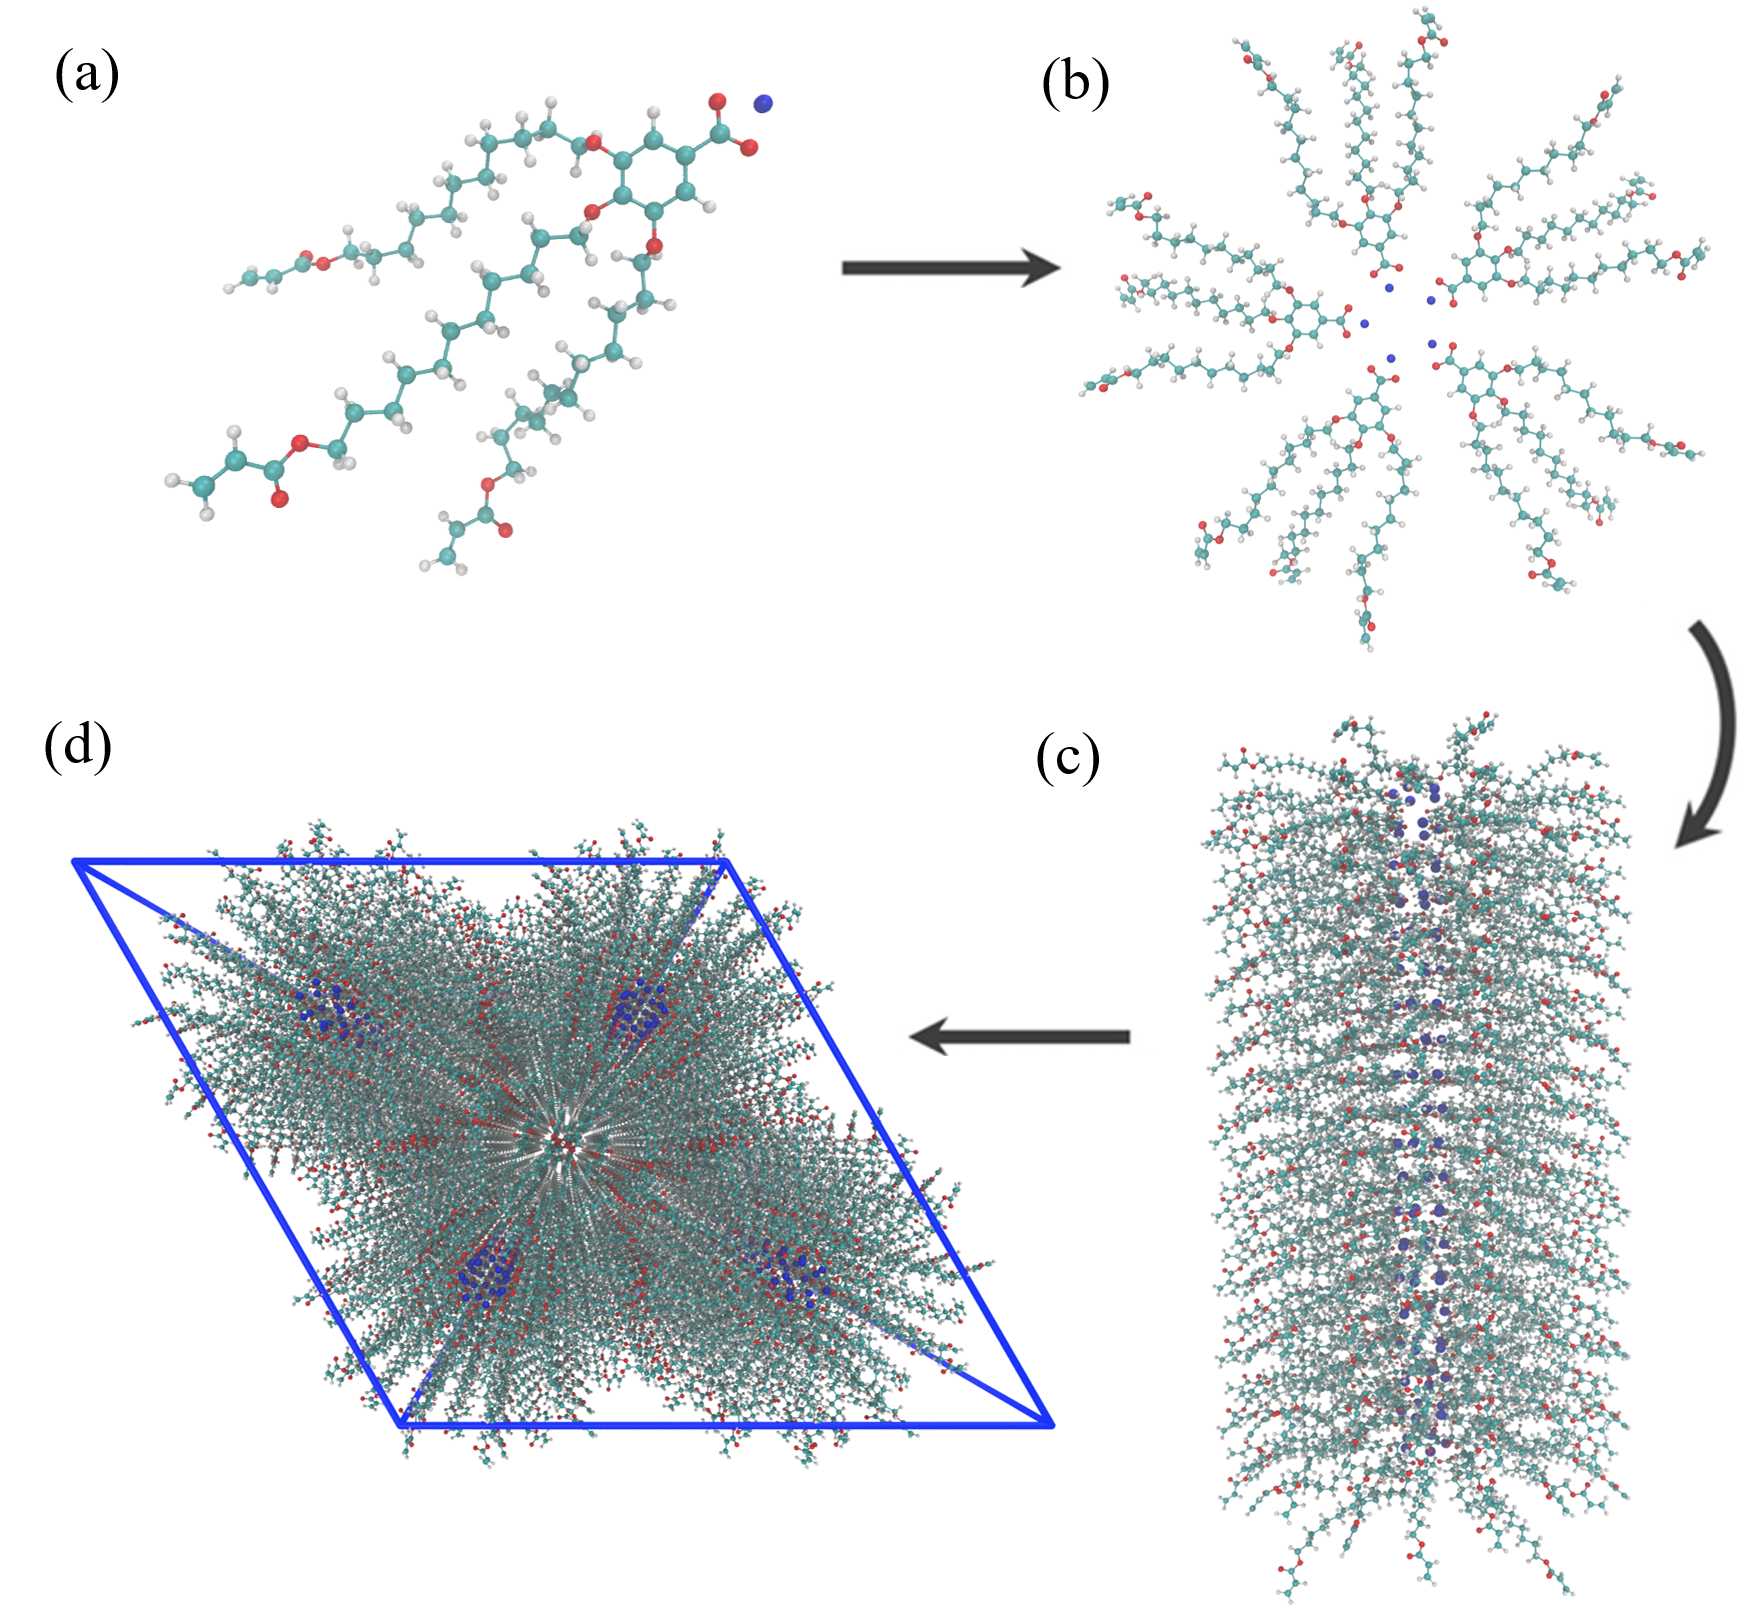
\includegraphics[width=0.75\linewidth]{build.PNG} %BJC: put an xyz axis with the unit cell
	\caption{(a) A single monomer was parameterized and annealed to produce a low energy
		configuration. (b) Monomers are rotated and assembled into layers with 
		hydrophlic centers. (c) Twenty layers are stacked on top of each other to create
		a pore. (d) Pores are duplicated and placed in a monoclinic unit cell}\label{fig:python}
  \end{figure}
  
  A typical simulation volume contains four pores in a monoclinic unit cell,
  the smallest unit cell that maintains hexagonal symmetry when extended 
  periodically.
  \begin{itemize}
    \item Each pore is made of twenty stacked monomer layers with periodic 
    continuity in the z direction, avoiding any edge effects and creating an 
    infinite length pore ideal for studying transport.
    \item A small number of layers is preferred in order to reduce computational
    cost and to allow us to look at longer timescales.
    \item Ultimately, we chose to build a system with 20 monomer layers in each pore
    in order to obtain sufficient resolution when simulating X-ray diffraction patterns.
    This point will be explained in more detail later.
    %MRS: you should give the reasons in the same place you describe the choice, but the supporting data would probably be better in supporting information
    %BJC: so refer to supporting info here? Then put plots of diffraction data with different sized system there. I did not explain the resolution point here because I haven't talked about simulated X-ray diffraction yet and it wouldn't make sense. And it doesn't make sense to talk about XRD this early in the methods.
  \end{itemize}
  
  We chose initial guesses for the remaining structural parameters based on 
  experimental data and treated them as variables during model development.
  %BJC: I could potentially break this paragraph into smaller paragraphs centered around
  % the bolded structural parameters
  %MRS Breaking into more structure is good. Short sentences, only 3-5 sentences per paragraph.

    %MRS: initial distance between pores -- we set the initial, and let it find where it wants to be
    %MRS: Or is this the initial data we COMPARE to? Be more specific about the use of these numbers. The use of the data needs to be clarified, since it's main effort here. 
  We placed pores at a chosen initial spacing, then allowed the system to settle 
  into its preferred spacing. 
  \begin{itemize}
    \item Our chosen distance between pores was based on experimental SAXS data for
    this system \cite{feng_thin_2016}.
    %MRS: somewhere, should explain there's a large dependence of (meta)stable structures based on this initial distance.  It's sort of important to put somewhere.
    %BJC: Sure, but different choices of pore spacing were based on number of monomers per layer. More monomers per layer means a larger initial pore spacing.
    \item The model's pore centers are spaced 4.5 nm apart initially, $\approx$ 10 \% larger
    than the experimental value of 4.12 nm in order to reduce unintended repulsions 
    resulting from a tightly packed initial configuration.
    \item To calculate the equilibrated pore spacing, we measured the distance between pore
    centers.
    \item Pore centers were located by averaging the coordinates of sodium ions in their 
    respective pores.
    \item Statistics were generated using the bootstrapping technique.
    %BJC: Do bootstrapping details go in supplemental?
    \item For each bootstrap trial, we recreate an equilibrium trajectory by randomly 
    sampling from the original trajectory
    \item Each pore spacing has its own trajectory with its own average value
    \item The average value of each pore spacing is averaged to get the overall
    average pore spacing. 
    \item The standard deviation of average values is reported as the uncertainty in pore spacing
    % BJC: The following will go in supplemental
    \item We are interested in 5 pore-to-pore distances which should all be equal in 
    a perfect hexagonal array. Only 4 are independent  
  \end{itemize}
  
  %MRS: initial layer spacing.
  We chose a layer spacing based on experimental 2D WAXS data.
  \begin{itemize}  
    \item The pattern shows reflections corresponding to features spaced 3.7 \angstrom~apart.
    \item It has been hypothesized that the features are a result of pi-pi
    interactions between stacked aromatic rings \cite{feng_scalable_2014}. 
    \item Our simulations tend to equilibrate to a wider interlayer spacing of
    $\approx$ 4.1 \angstrom, which inspired separate systems starting with layer 
    spacings greater than 4 \angstrom.
  \end{itemize}
    
  %MRS: pore radius is a different category isn't it? Is this an input piece of data?
  % should be put in a different category.
  %BJC: Well I still have to initially place the monomers some distance away from the pore
  % centers. That distance is informed by the experimental evidence.
  
  We based the pore radii of our initial configuration on past TEM and size exclusion 
  rejection data
  We used experimental Transmission electron microscopy (TEM) and size exclusion rejection
  data \cite{feng_scalable_2014,feng_thin_2016,zhou_supported_2005} to inform our definition
  of pore radius in the initial configuration.
  \begin{itemize}
    \item Experimental evidence suggests uniform pores with radii of 0.6 nm a pore radius
    \item Comparing a geometric measurement of pore size derived from an 
    atomistic model, to a less precise, experimentally derived pore size estimate,
    will give ambiguous results.
    \item What is meant by pore radius will not be clear until we have a clear picture
    of the nanoscopic pore environment.
    \item Atomistic simulations do a good job of providing the level of detail we need. The challenge
    will be to ensure that we are producing the correct picture.
    %MRS: point out this is one of the things that atomistic simulation can actually do very well - 
    % provide a clear picture of a nanoscopic environment (the questions is whether it's 
    % providing the _right_ clear picture).
    \item When constructing pores, we chose the carboxylate carbon from the monomer
    head group as a reference atom, and placed it a distance r from the pore center,
    where r is the pore radius.  %BJC: figure making that clear
    \item We will not make direct comparisons of pore radius between our model 
    and experiment to avoid the ambiguity. 
    \item However, we do define a pore radius based for our own purposes.
    \item Pore radius was measured by calculating the distance between the center of 
    mass of each aromatic ring and the center of mass of all aromatic rings in their 
    respective pores.
  \end{itemize}
  
  %MRS: OK, this is a variable again that we need to set. 
  The \textbf{relative interlayer orientation} was chosen based on clues from 
  diffraction data as well as the various known stacking modes of benzene 
  and substituted benzene rings: sandwiched, parallel-displaced and T-shaped
  ~\cite{sinnokrot_estimates_2002} (\Cref{fig:sandwiched,fig:pd,fig:tshaped}).
  \begin{itemize}
    \item The T-shaped configuration was ruled out based on the inconsistency of
    its $\approx$ 5 \angstrom~equilibrium stacking distance ~\cite{sinnokrot_estimates_2002}.
    \item The system's preference towards the sandwiched vs. parallel displaced 
    stacking modes will be explored.
    %BJC: I think the following commentary belongs elsewhere, maybe even in the discussion
    %MRS: hard to say. It's certainly a big switch from things that are relatively straightforward to things that require 
    % a fair amount of information, so I think it belongs in it's own section -- so far, you're just laying out the approach.  This is what we fix, this is what we leave as a variable.  The analysis probably belongs later.
    %BJC: Yeah, I will leave the rest for discussion
%     \item Visualization of each configuration (\Cref{fig:sandwichedlayers,fig:offsetlayers})
%     suggests entropic differences based on the way the tails are able to pack.
%     \item In the sandwiched configuration, all tails start out directly on top
%     of each other which may prevent closely stacked benzene rings.
%     \item In the offset configuration, the tails are placed in between each other 
%     which may allow layers to come together in a compact way.
%     \item This difference may explain, in part, which stacking mode is more favorable.
  \end{itemize}

  An equilibration scheme with position restraints placed on aromatic rings
  %MRS: 
  %prevents 
  during early equilibration steps is required to prevent high energy repulsions .
  %MRS: should be clearer what you mean by ``unrealistic jumps''.  Hard to visualize.
  %BJC: 'high energy repulsions' ?
  \begin{itemize}
    \item Restraints fix monomer head groups in the sandwiched or parallel-displaced
    configurations while allowing monomer tails to settle.
    \item Doing so also mitigates system dependence on initial monomer configuration.
    \item The restrained portion of the equilibration scheme is run in the NVT ensemble.
    \item Every 50 ps, we reduce the force constants by the square root of its 
    previous value, starting from 1e6 KJ mol\textsuperscript{-1} nm\textsuperscript{-2}.
    \item Once the force constant is below 10 KJ mol\textsuperscript{-1} 
    nm\textsuperscript{-2}, the restraints are slowly released until there is no more 
    restraining potential.  
    \item The resulting unrestrained structure is allowed to equilibrate further in the NPT
    ensemble for 400 - 500 ns.
   %BJC: I will reference an equilibration script that can be released with the supplemental info
   %MRS: we should release as many scripts as is feasible, can be in a github repository.
   %BJC: Okay, once we submit, I will need to spend some time cleaning the scripts
   %MRS: You've described two equilibration procedures (or two varieties of the same one?) - need to be crystal clear to the reader as to which is used where.
   %BJC: Yea I'm just saying that I do 50 ps restrained simulations in NVT ensemble and then once the restraints are gone I switch to NPT. I edited the language to try and make it clearer.
  \end{itemize}
  
  %BJC: the following paragraph will be replaced with something that Joe writes
  %MRS: sounds good.
  Simulated X-ray diffraction patterns were generated based on atomic
  coordinates for a direct experimental comparison.
  \begin{itemize}
    \item All atomic coordinates were simulated as gaussian spheres of electron
    density corresponding to each atom's atomic number.
    \item A three dimensional fourier transform (FT) of the array of electron 
    density results in a three dimensional structure factor which represents
    the unit cell in reciprocal space.
    \item We perform an angular average of the structure factor about the 
    z axis to generate a 2D cross section close to what one would see 
    experimentally.
    \item We matched experimental 2D WAXS patterns by iterative improvement
    of our choice of initial structure and equilibration procedure.
  \end{itemize}
  
  \begin{figure}[!ht]
	\centering
	\begin{subfigure}[b]{0.32\textwidth}
		\centering
		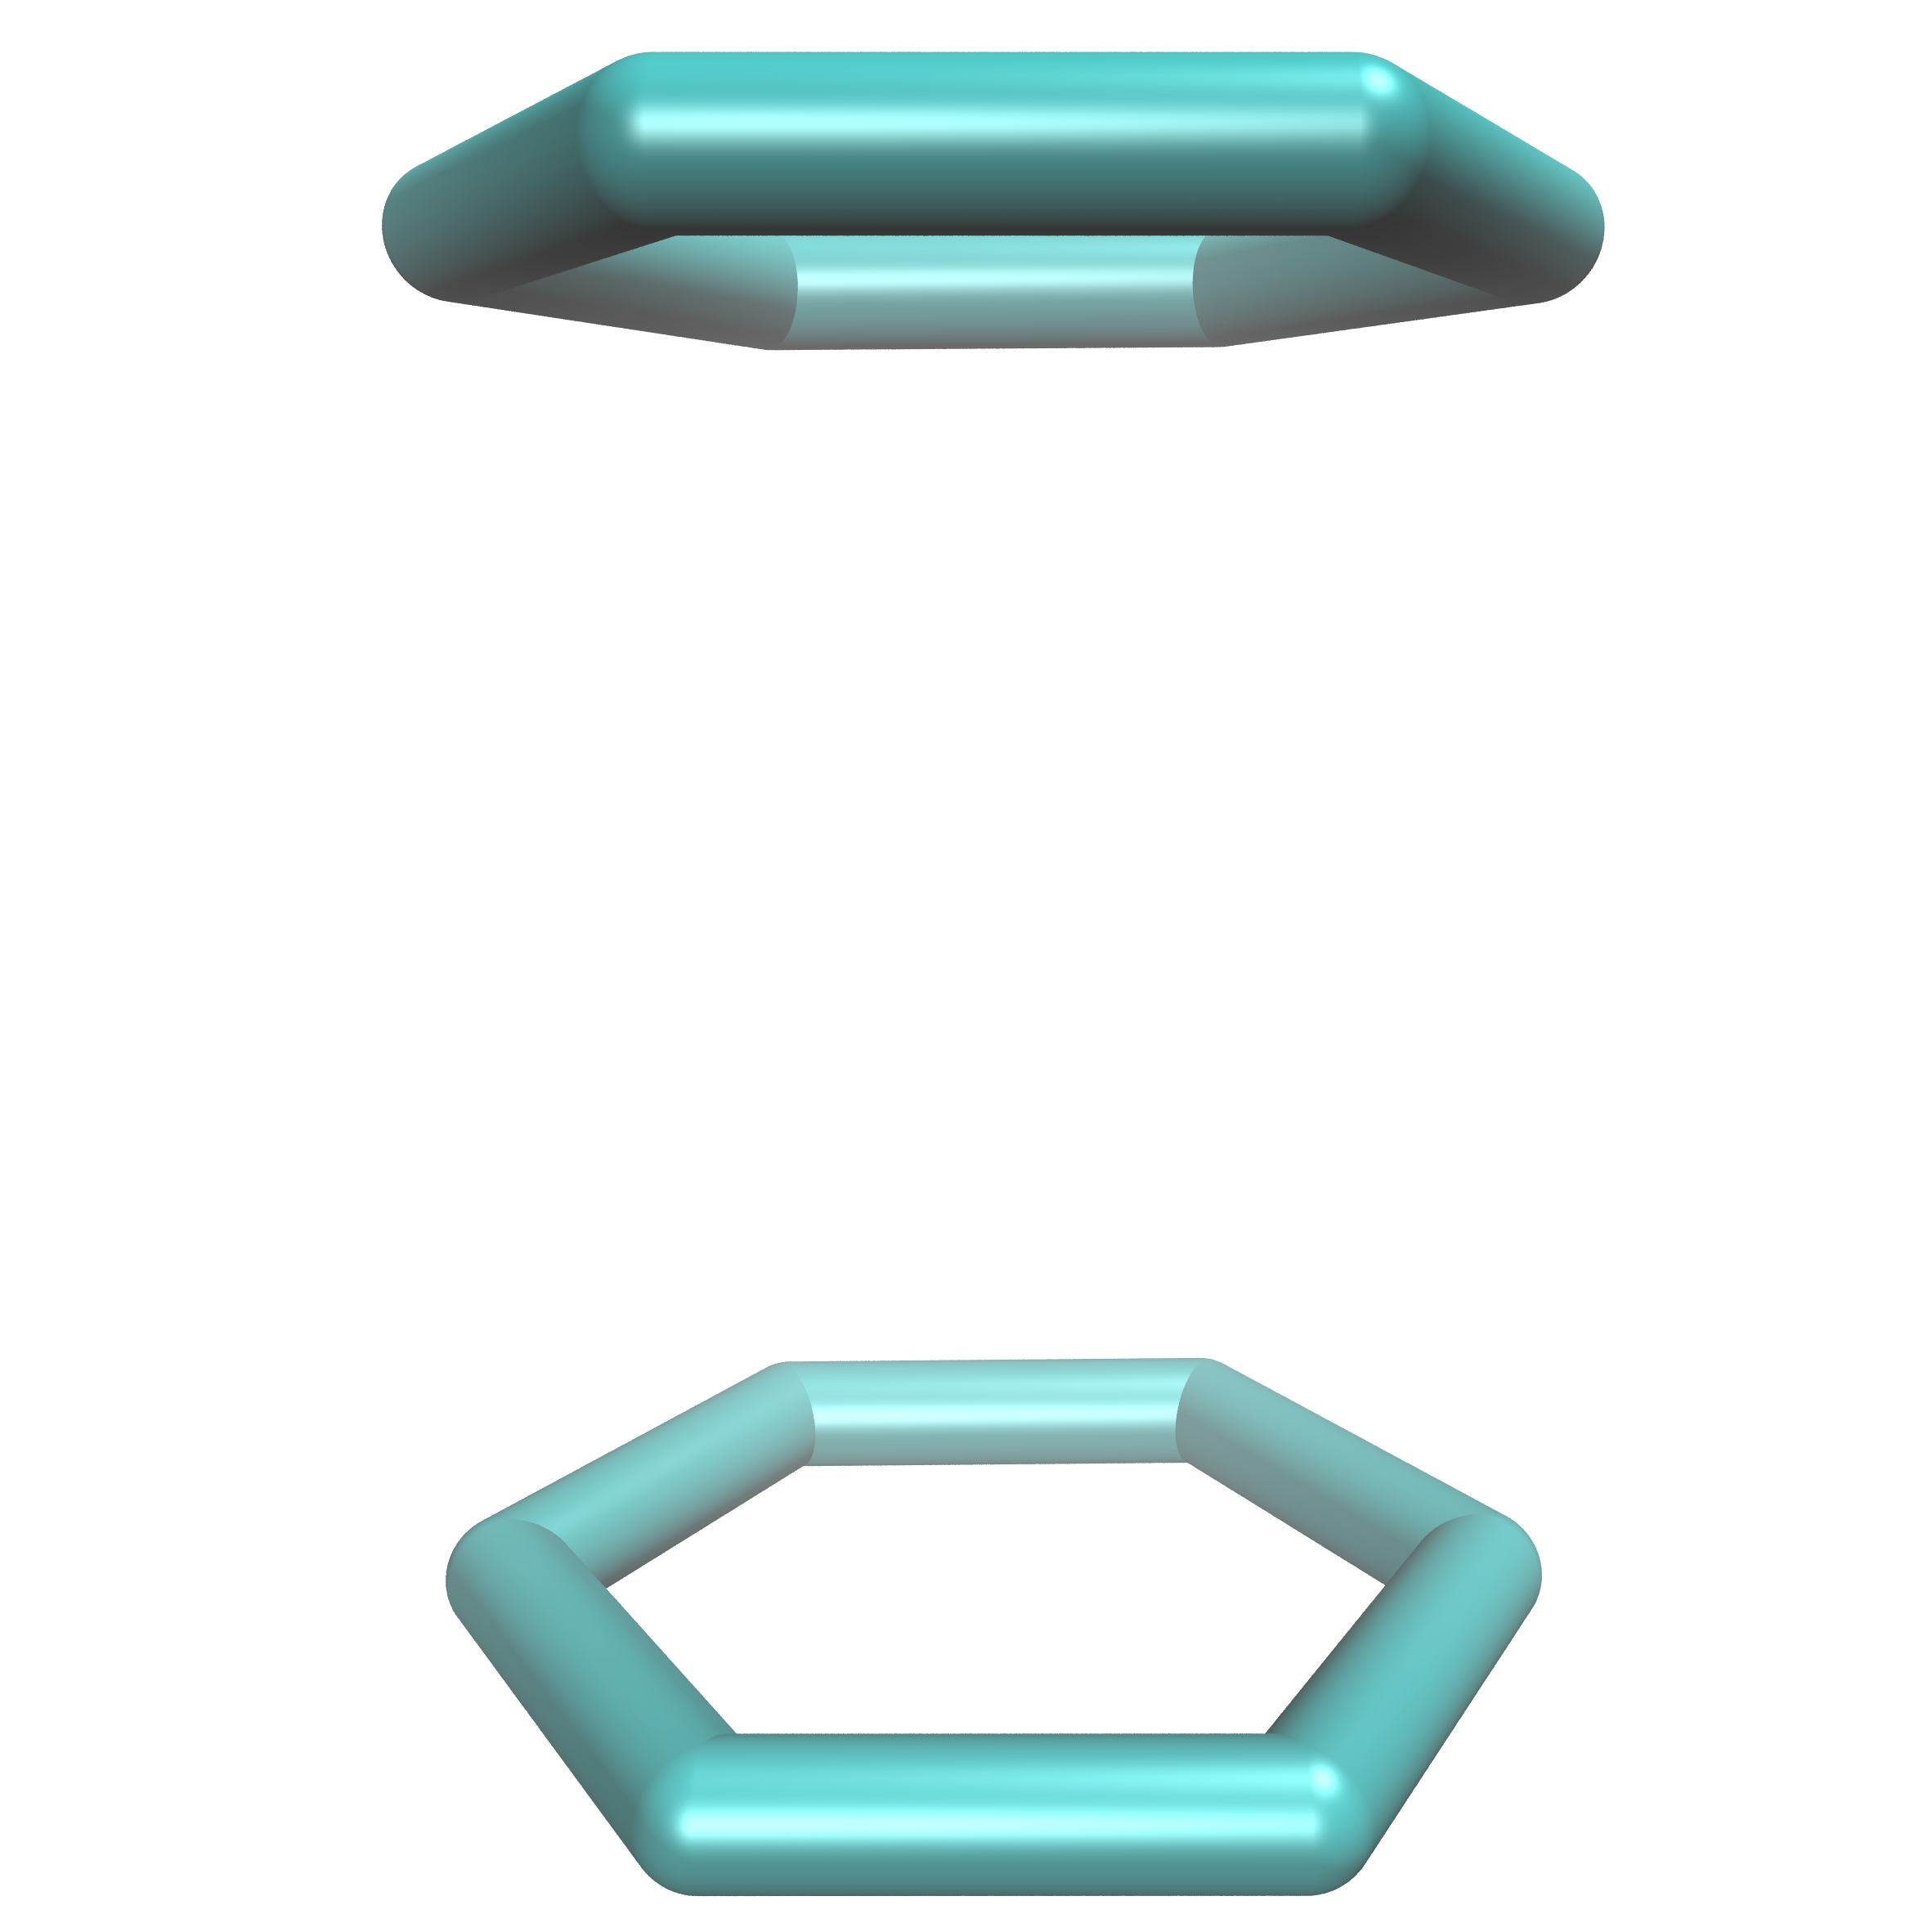
\includegraphics[width=\textwidth]{sandwiched.png}
		\caption{}\label{fig:sandwiched}
	\end{subfigure}
	\begin{subfigure}[b]{0.32\textwidth}
		\centering
		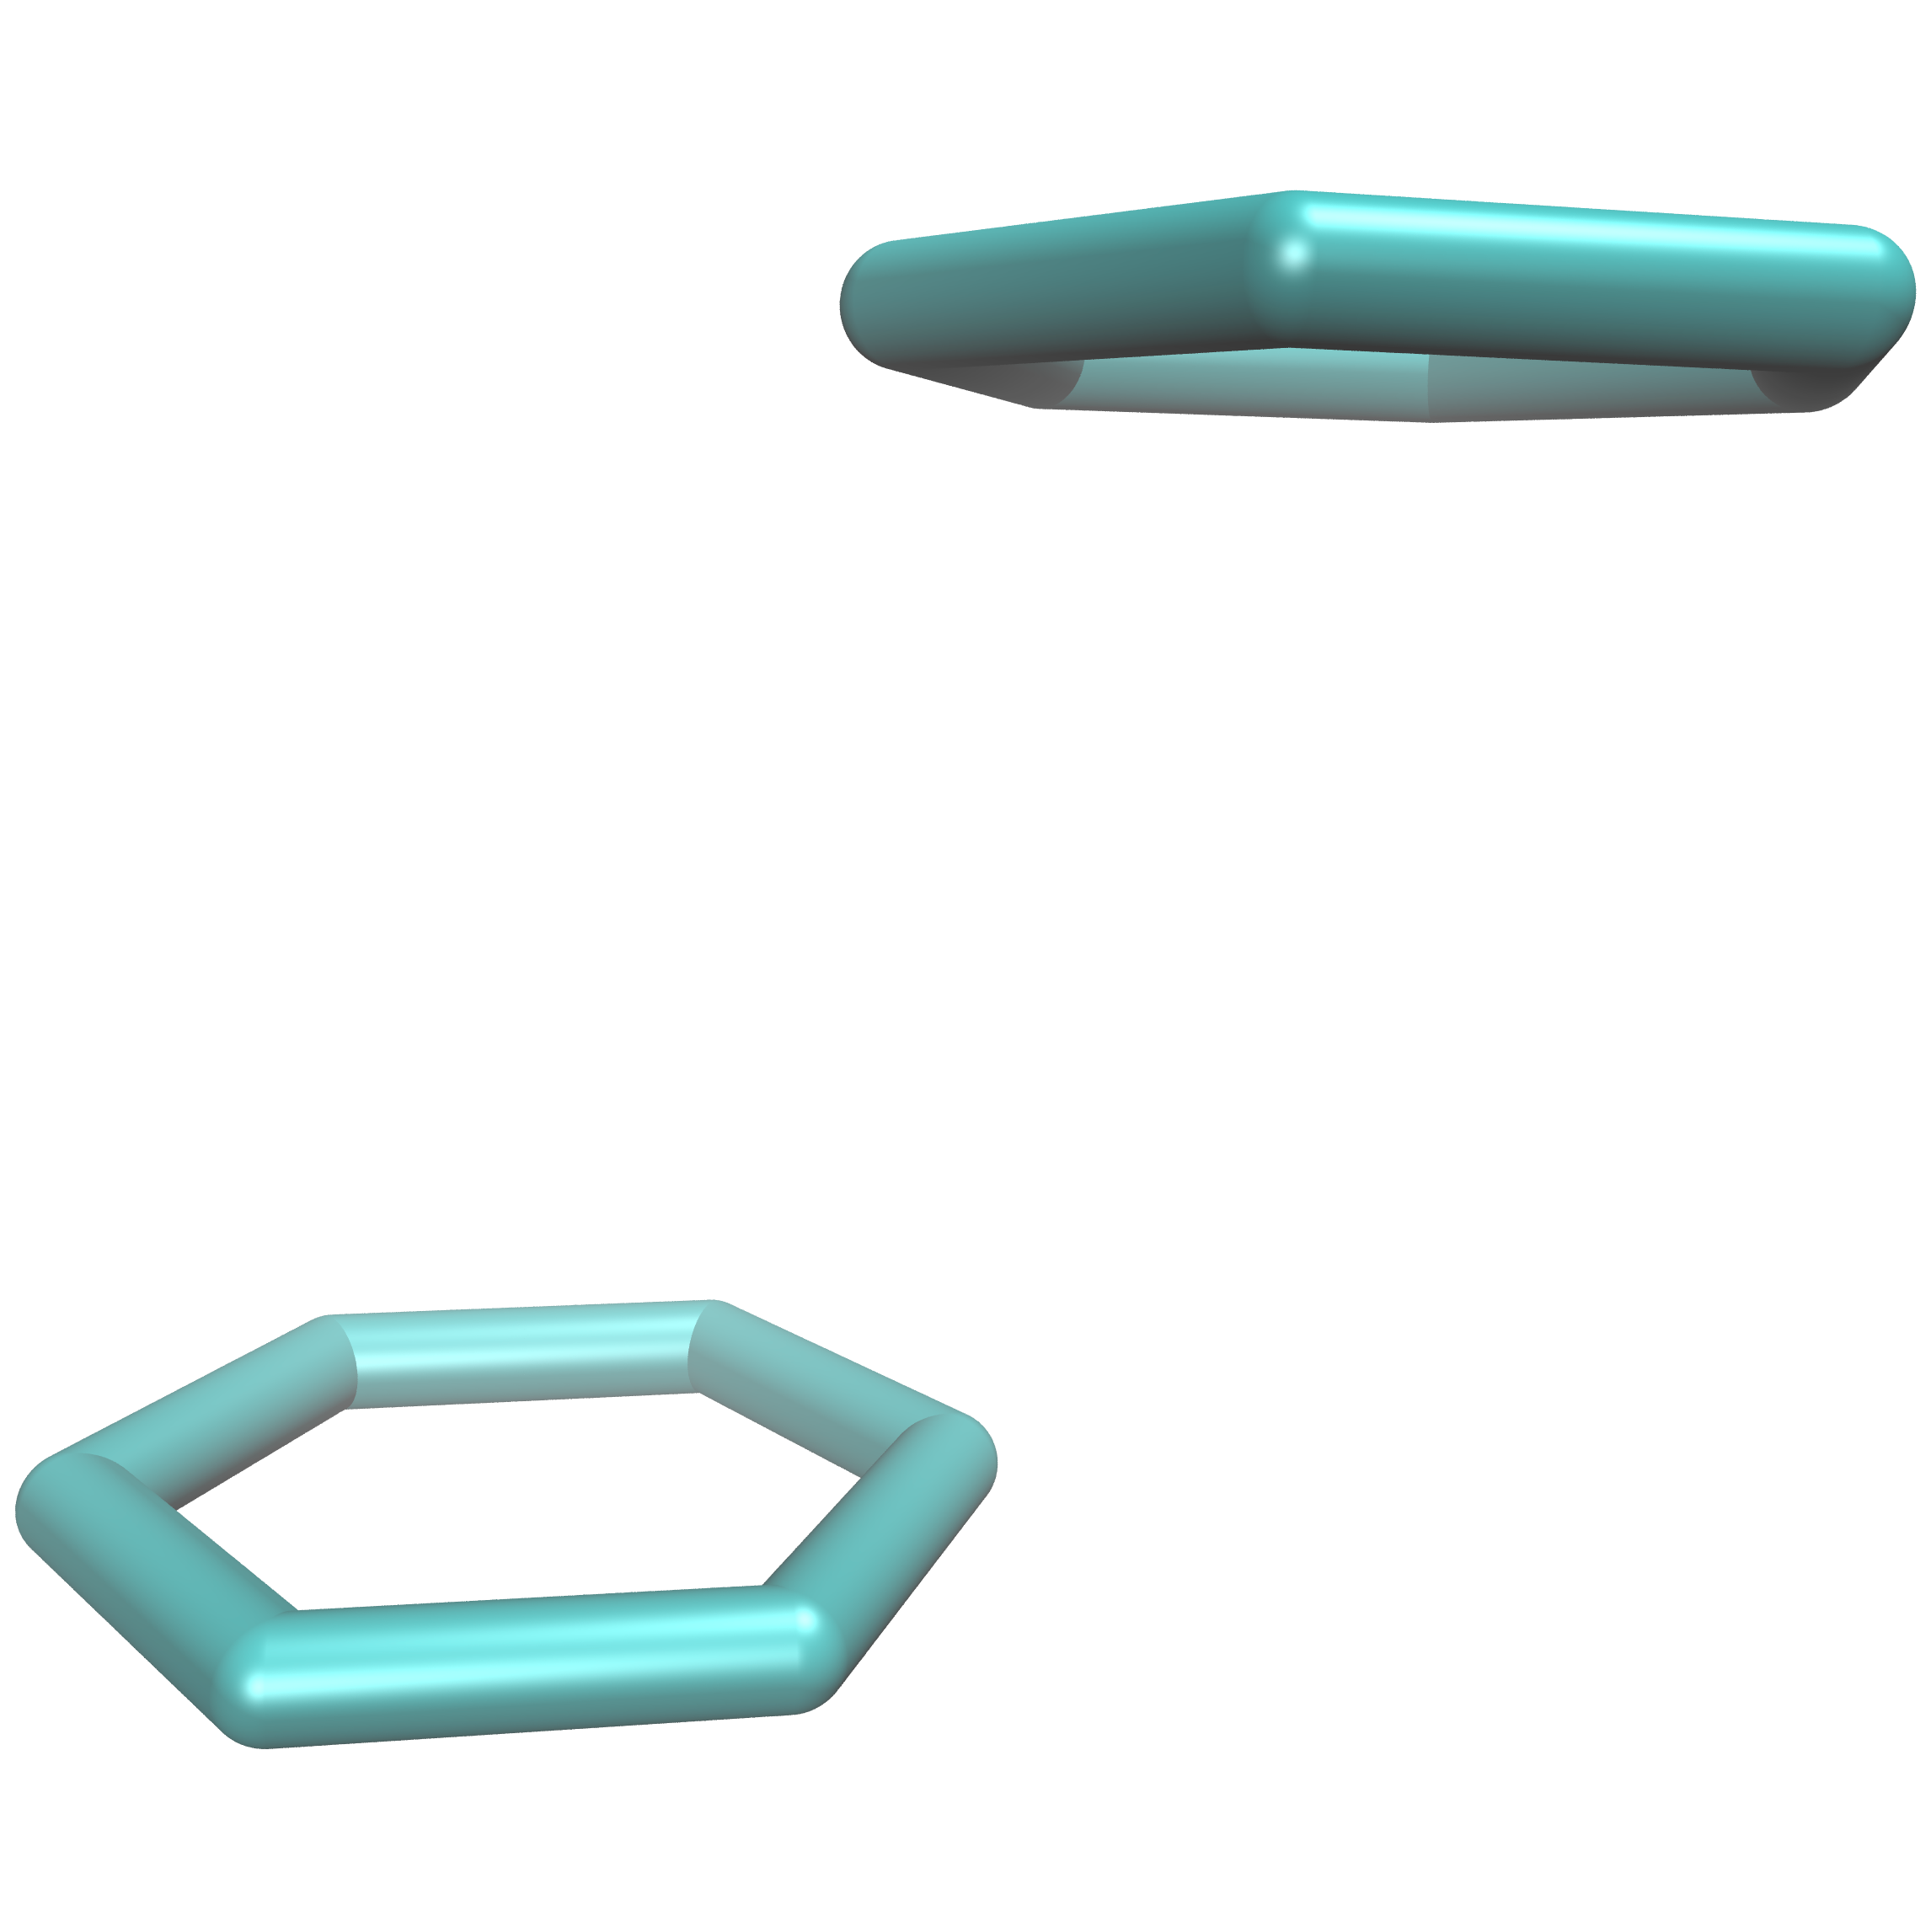
\includegraphics[width=\textwidth]{PD.png}
		\caption{}\label{fig:pd}
	\end{subfigure}
	\begin{subfigure}[b]{0.32\textwidth}
		\centering
		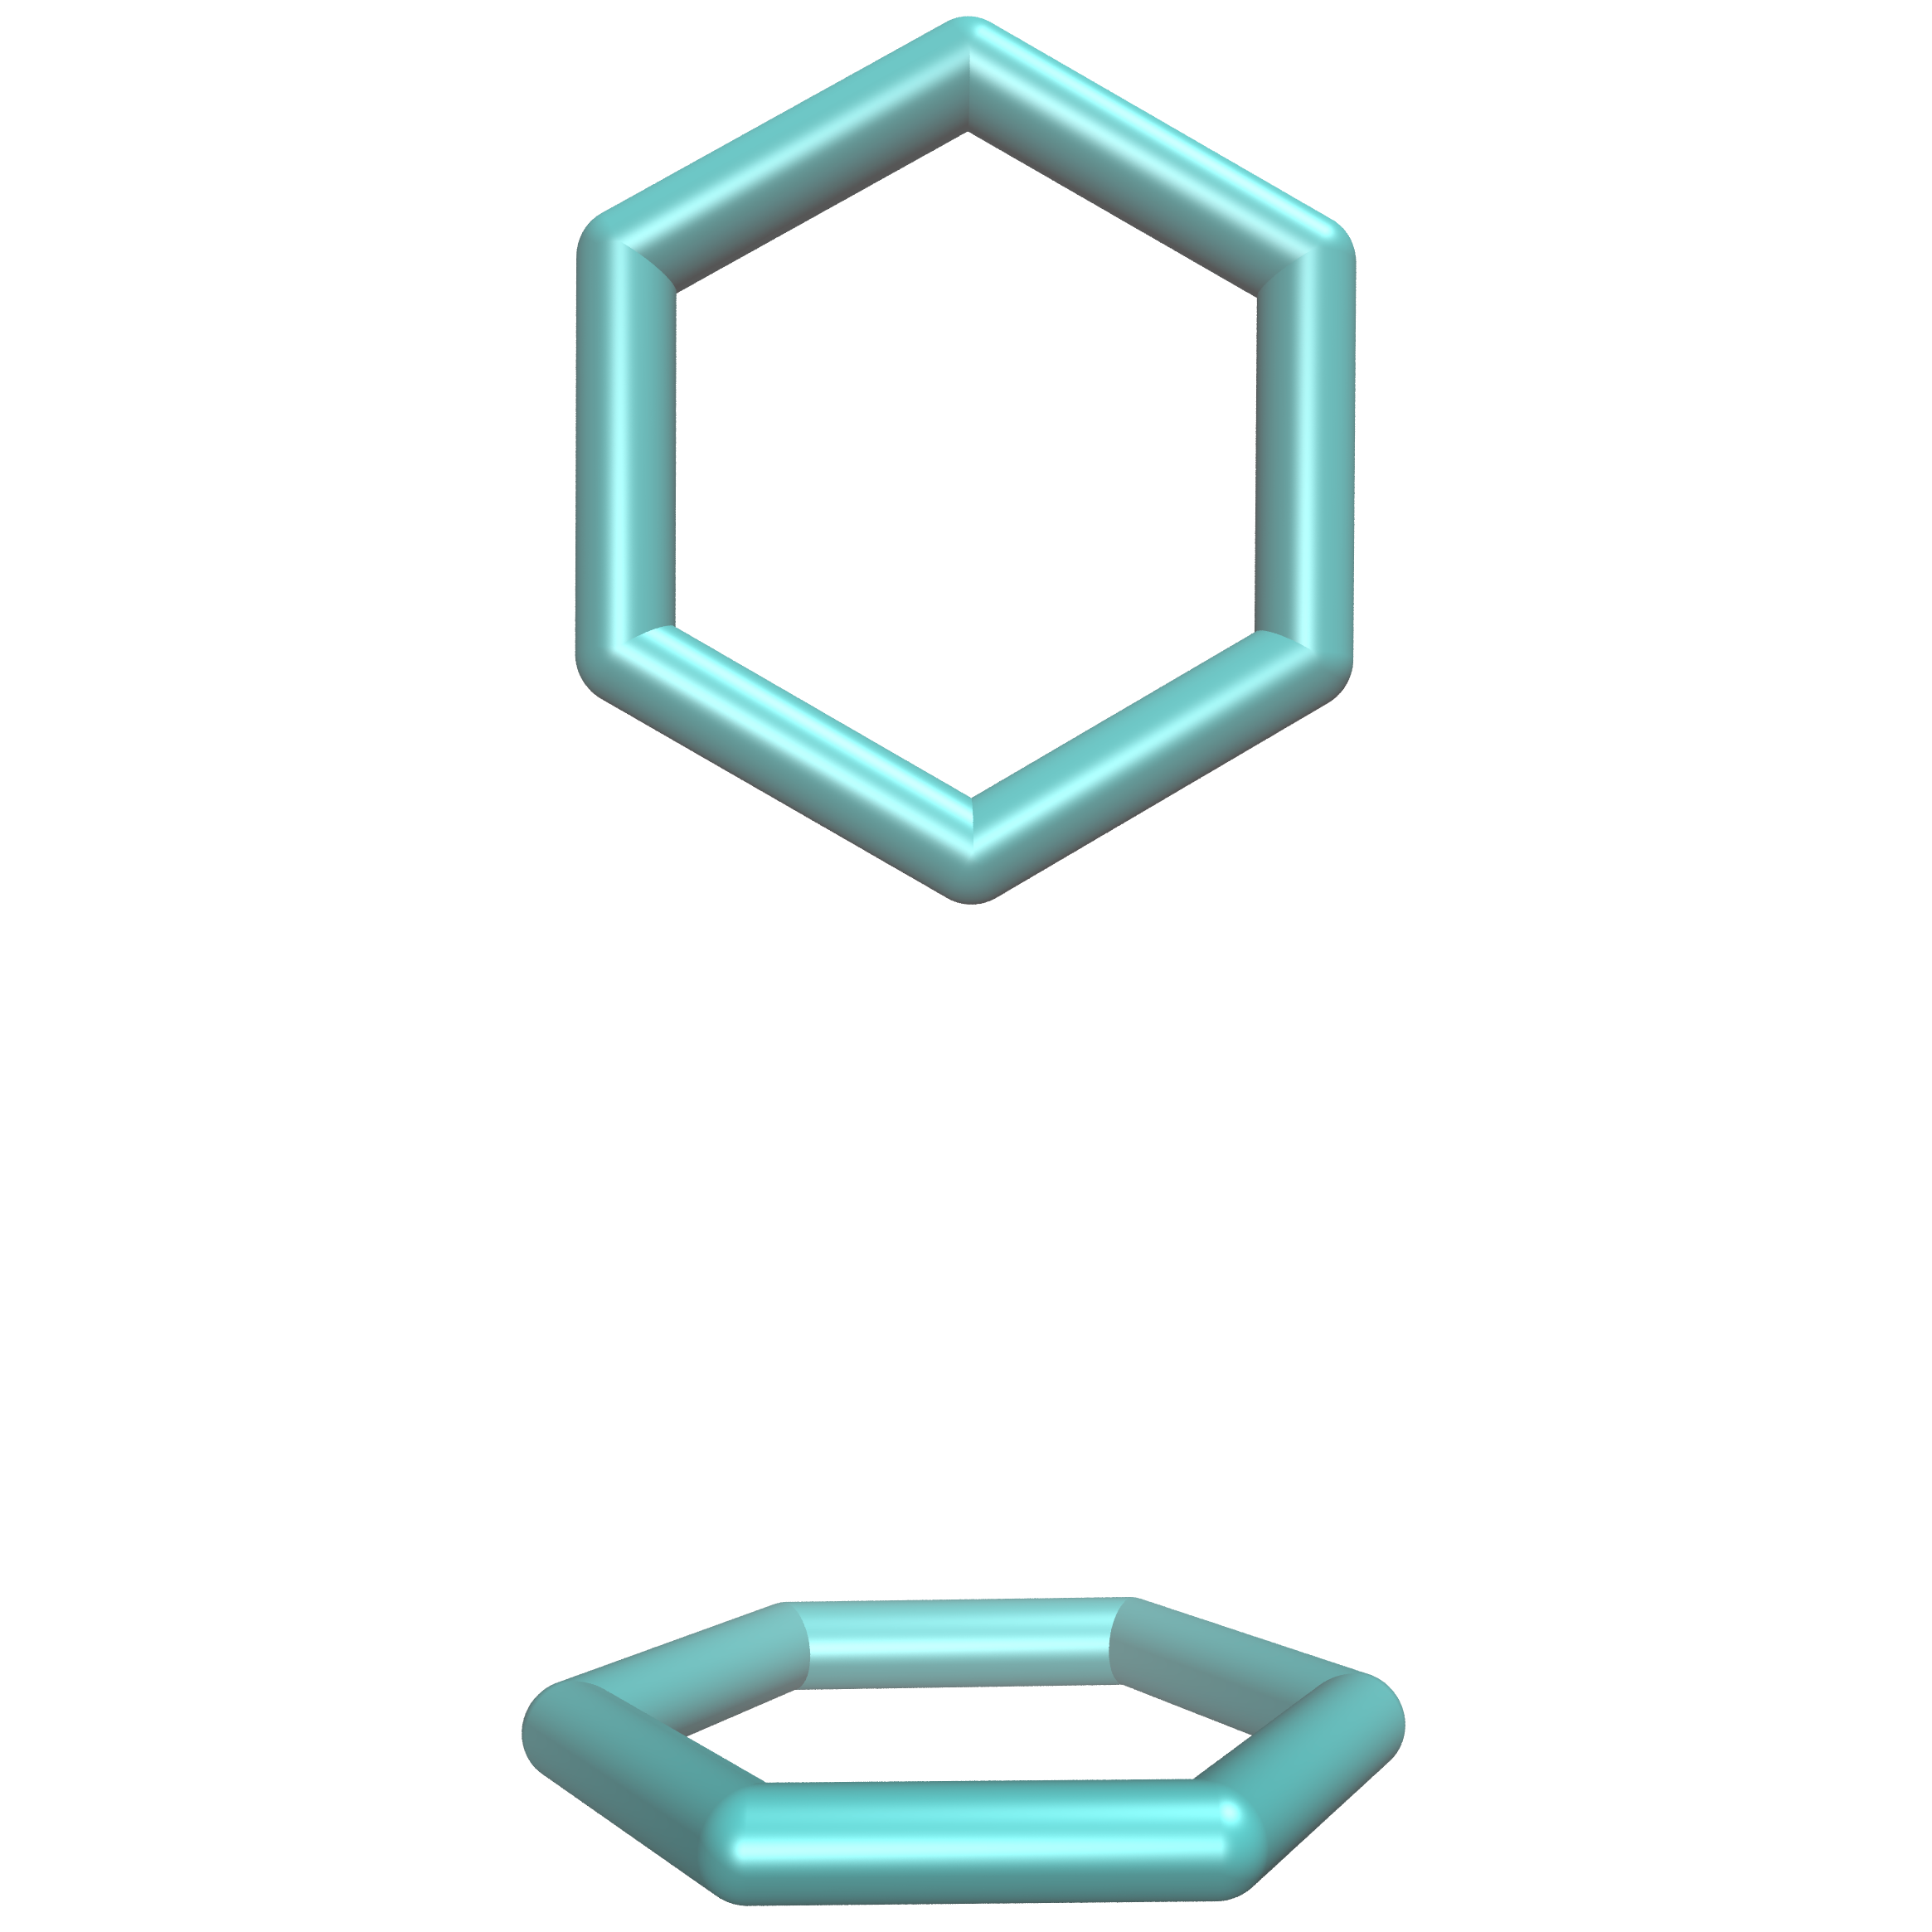
\includegraphics[width=\textwidth]{Tshaped.png}
		\caption{}\label{fig:tshaped}
	\end{subfigure}
	\vskip\baselineskip
	\begin{subfigure}[b]{0.475\textwidth}
		\centering
		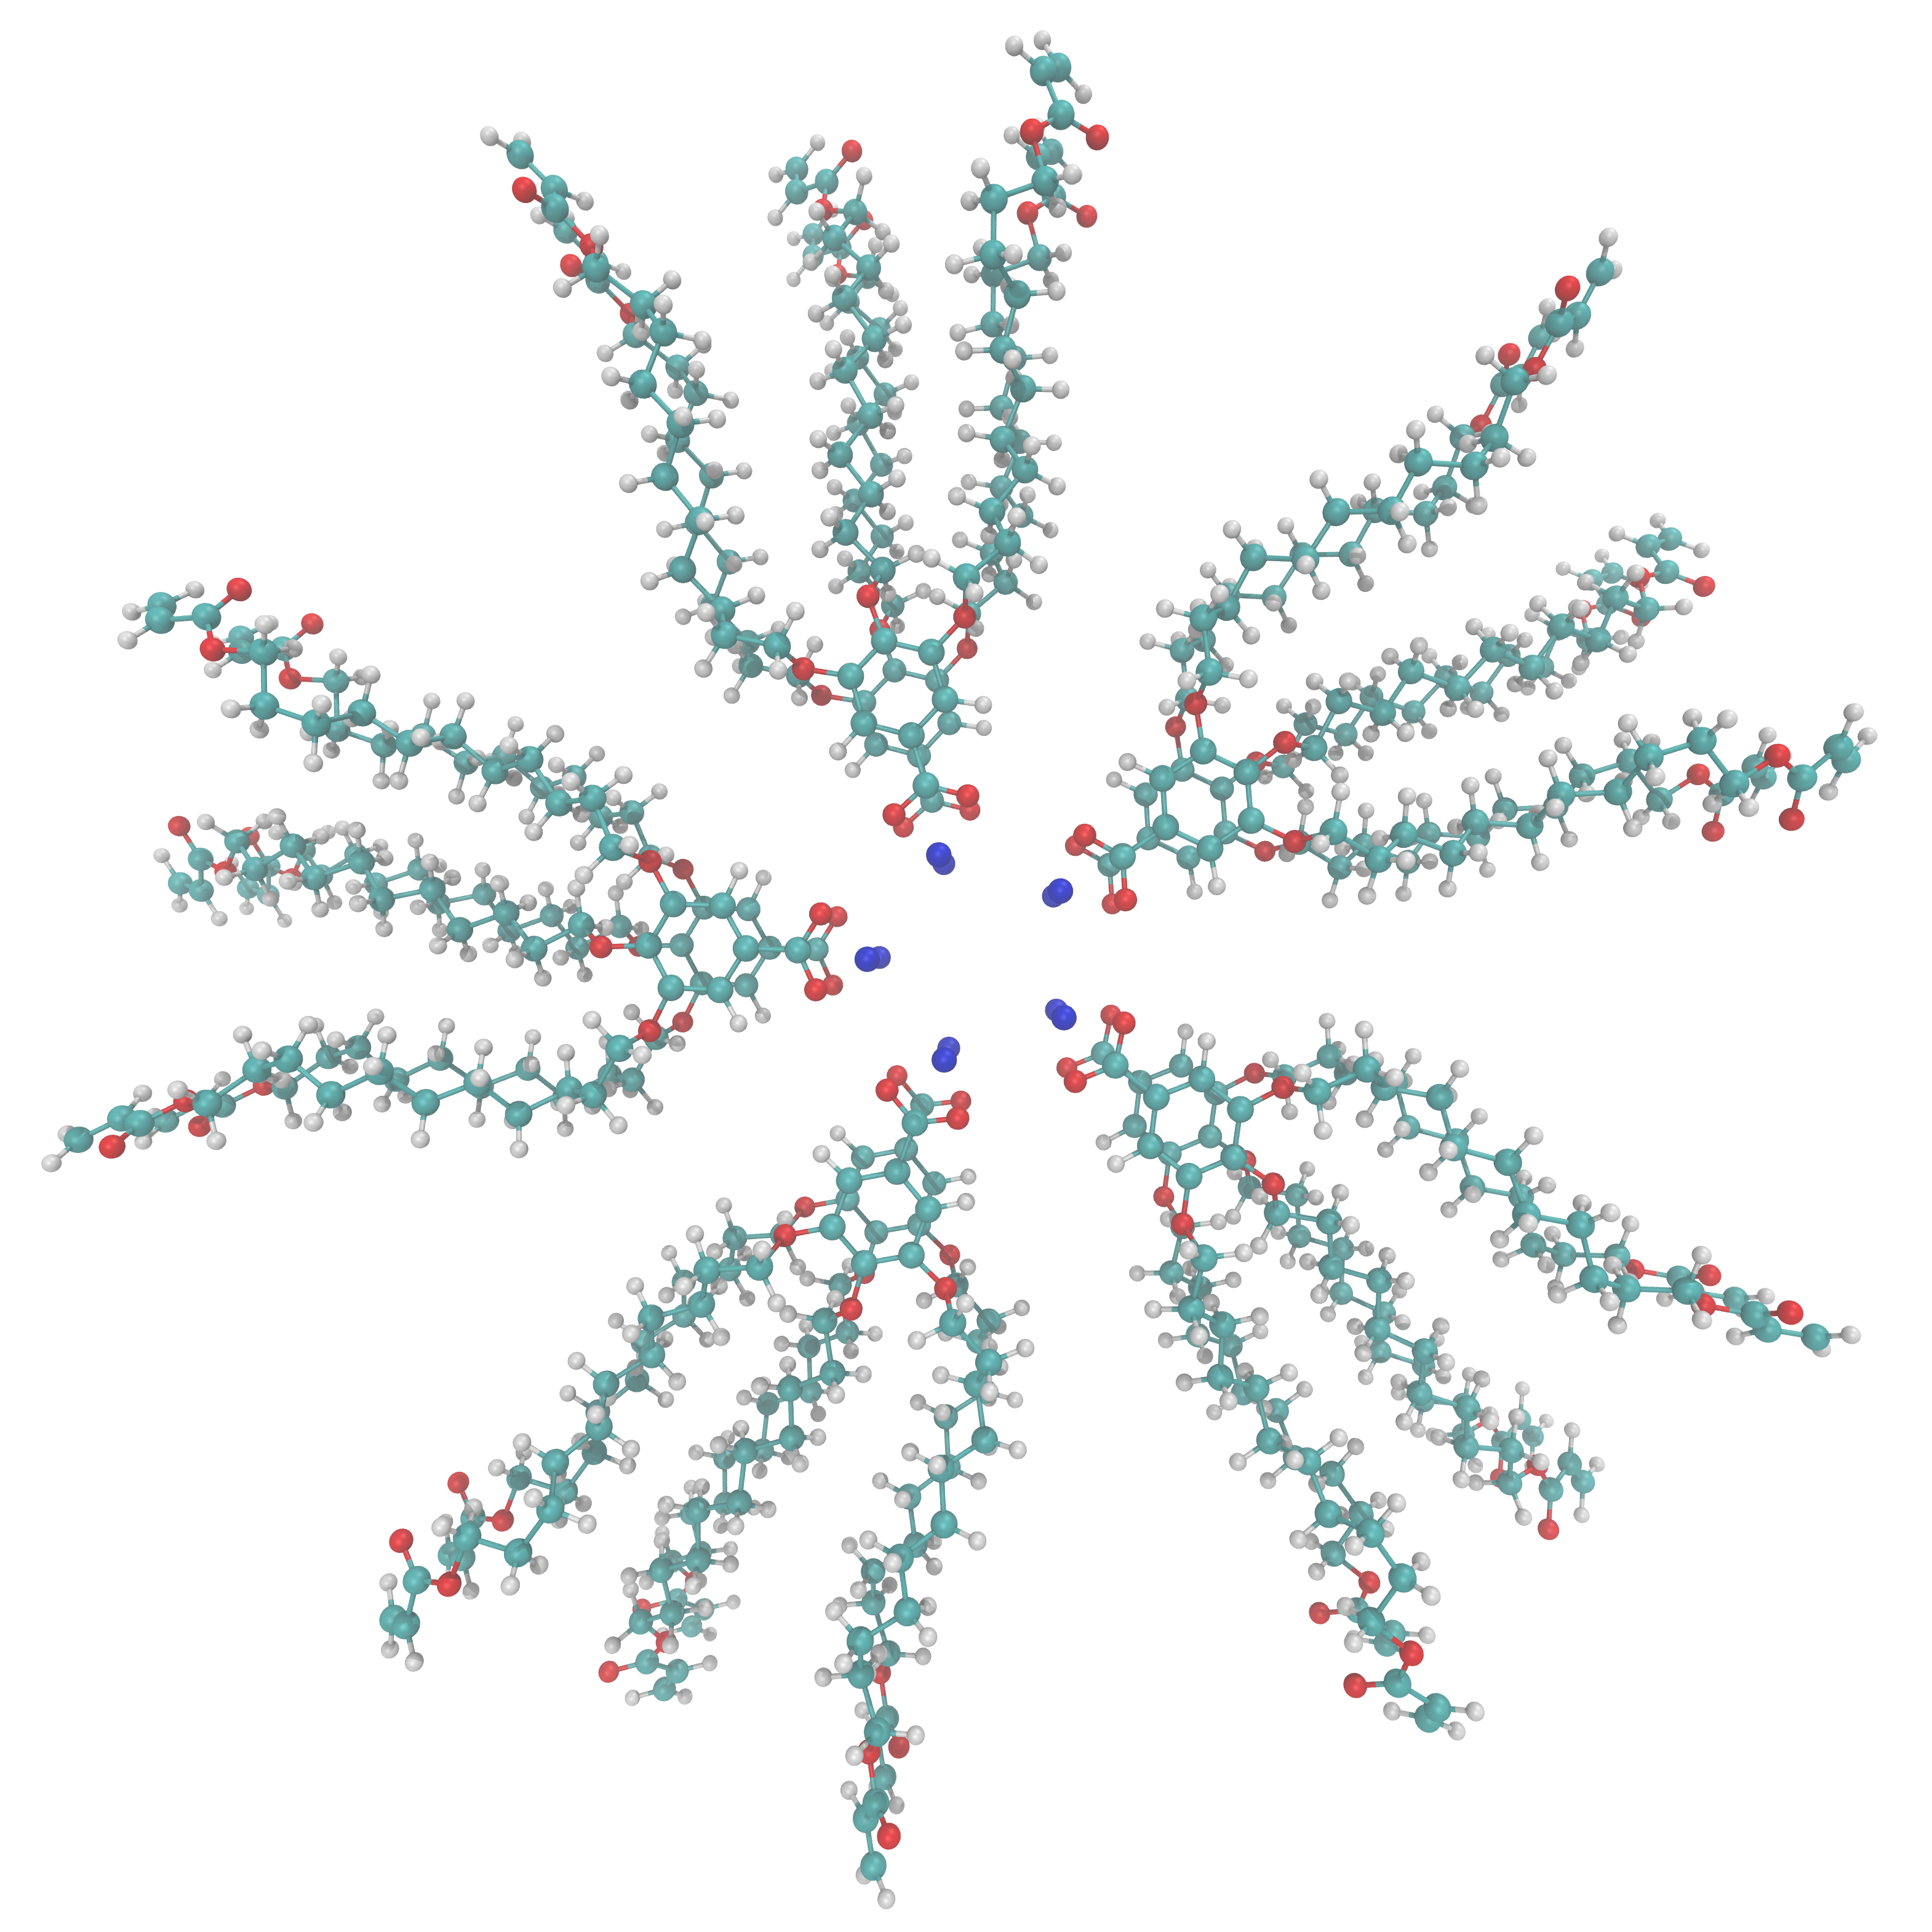
\includegraphics[width=\textwidth]{sandwichedlayers.png}
		\caption{}\label{fig:sandwichedlayers}
	\end{subfigure}
	\begin{subfigure}[b]{0.475\textwidth}
		\centering
		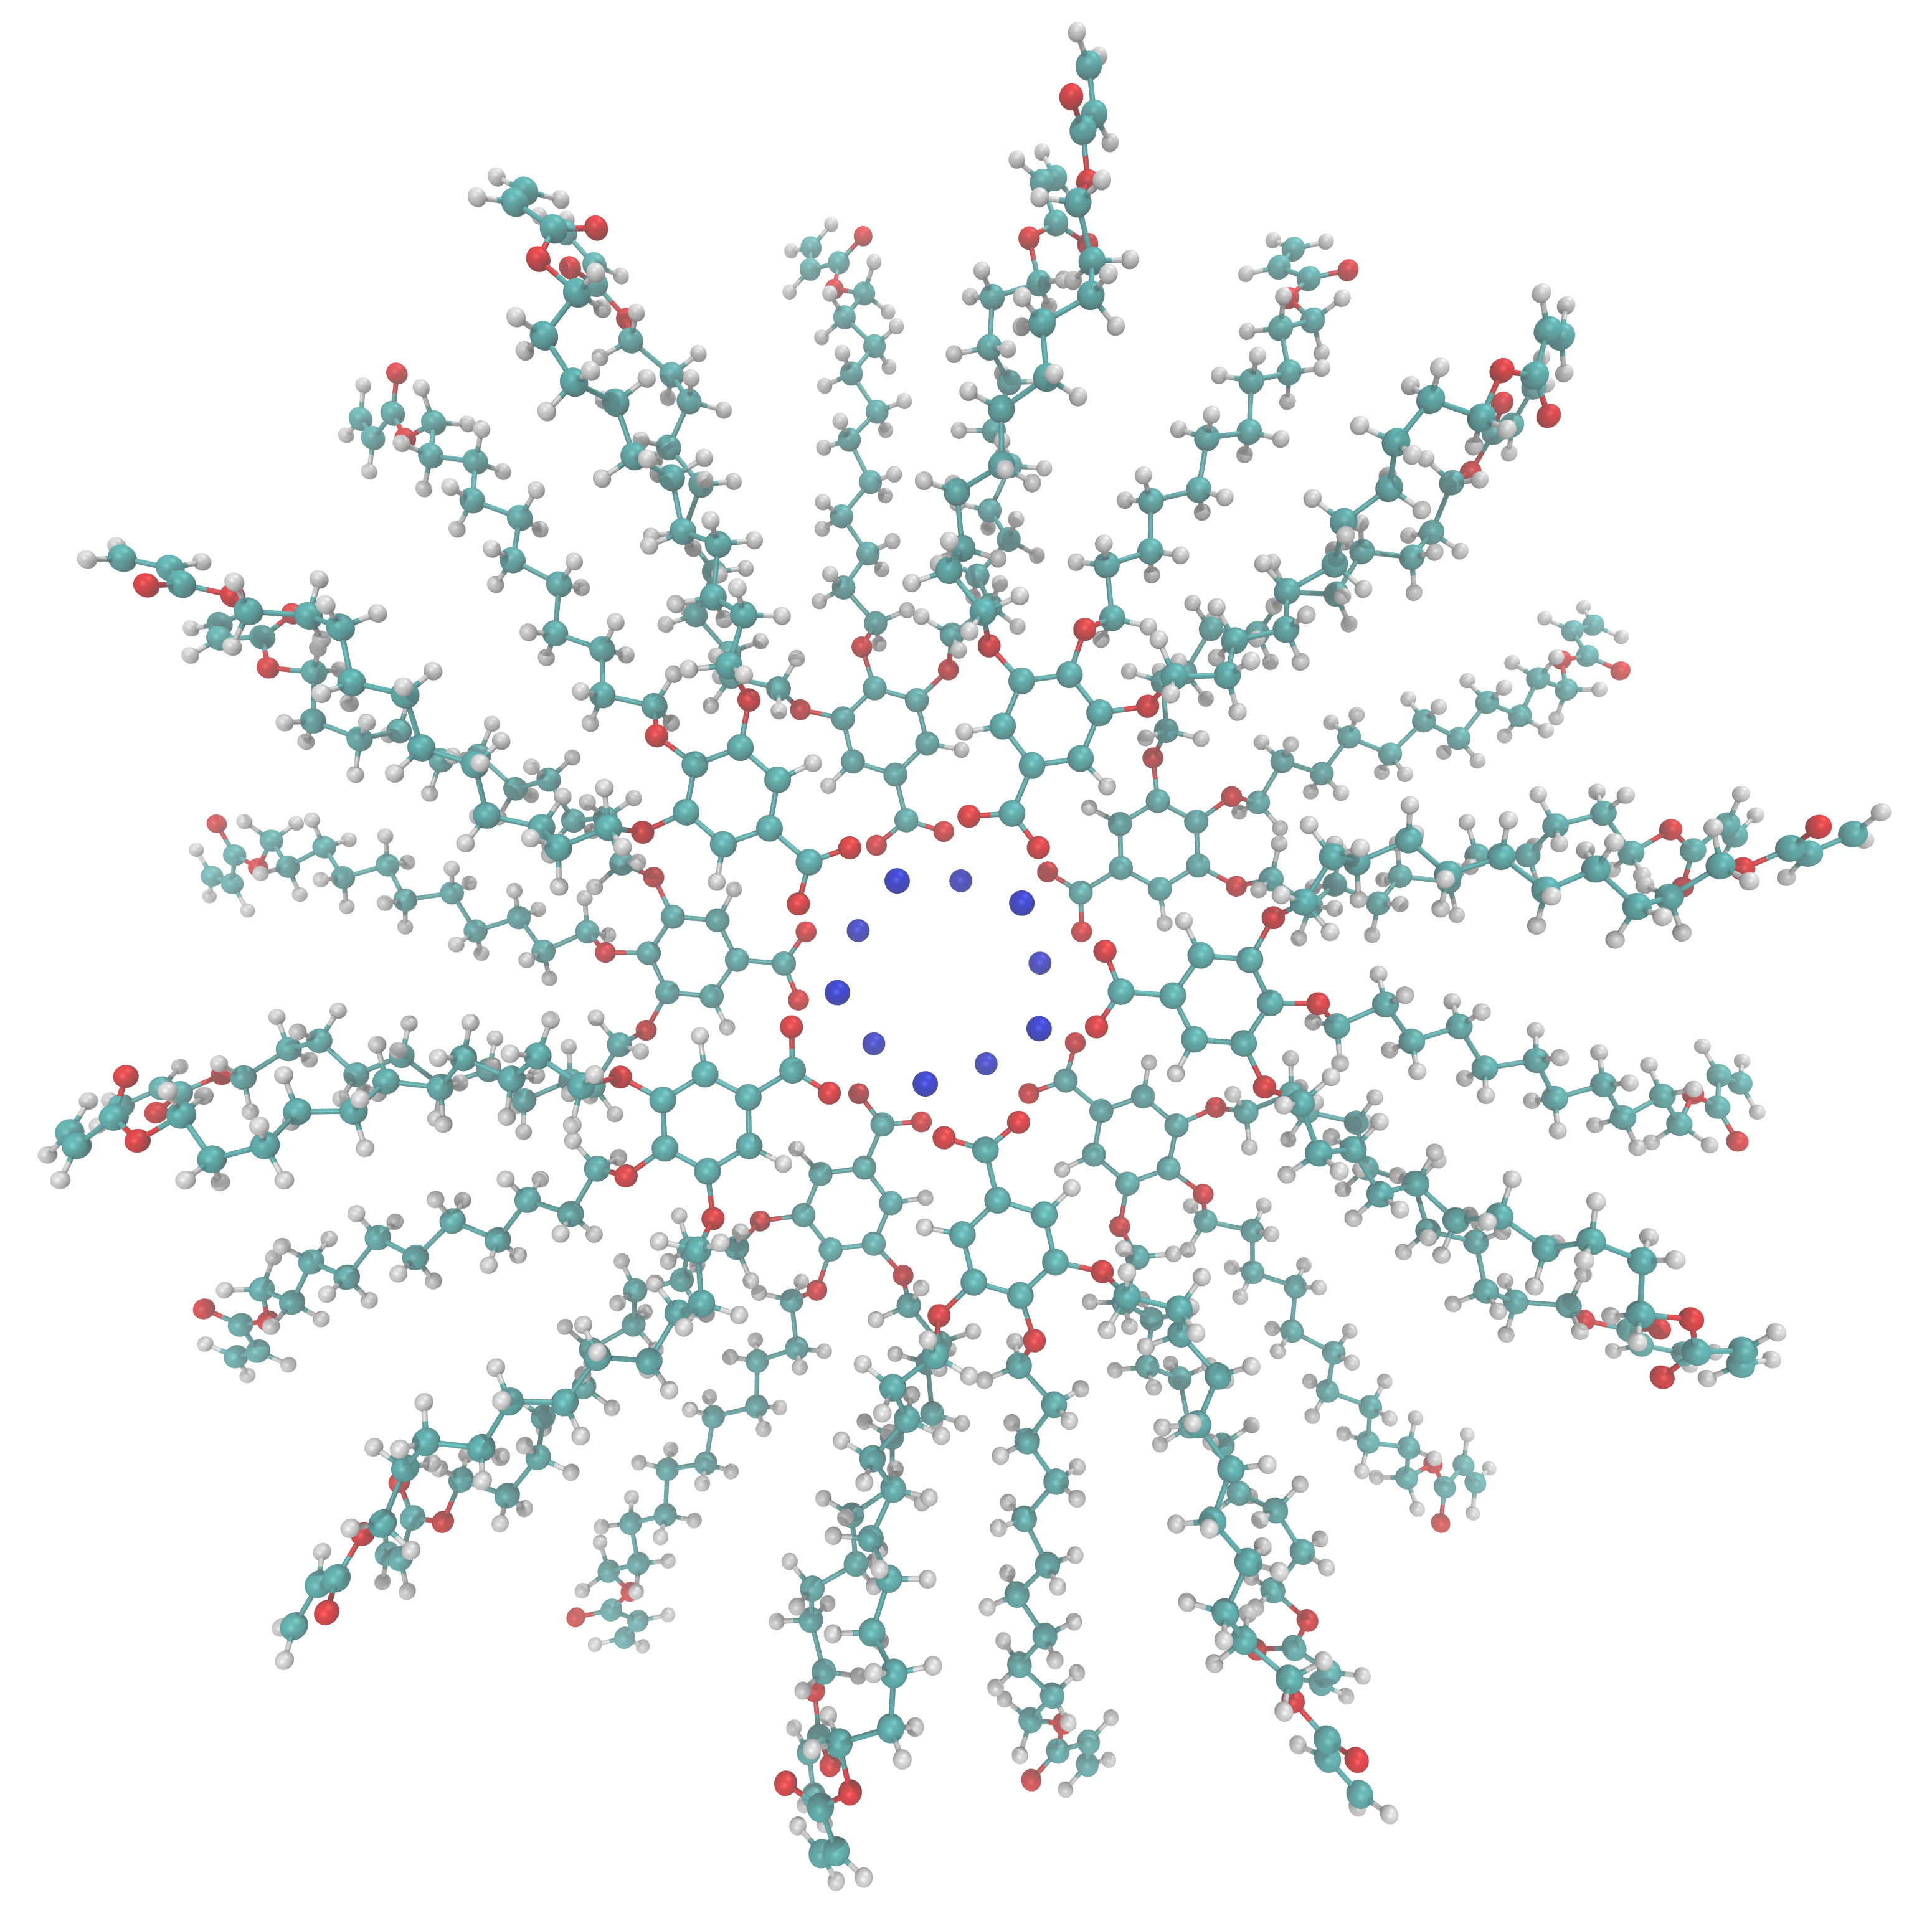
\includegraphics[width=\textwidth]{offsetlayers.png}
		\caption{}\label{fig:offsetlayers}
	\end{subfigure}
	\caption{(a) Sandwiched benzene dimers stack 3.8 \angstrom apart. (b) Parallel-Displaced benzene dimers stack
	3.4 \angstrom vertically and 1.6 \angstrom horizontally apart. (c) T-shaped benzene dimers stack 5.0 \angstrom apart. 
	(d) Two monomer layers stacked in the sandwiched configuration (e) Two monomer layers stacked in the parallel-displaced
	configuration }\label{fig:stacking}
  \end{figure}
  
  We calculated ionic conductivity using two different methods for robustness.
  \begin{itemize}
    \item The Nernst-Einstein relation relates the DC ionic conductivity to 
    ion diffusivity, $D$, concentration, $C$, ion charge, $q$, the boltzmann 
    constant, $k_b$, and temperature, $T$: $$\sigma = \dfrac{q^2CD}{k_b T}$$  %BJC: need citation
    \item Sodium ion diffusion coefficients were found by calculating the slope
    of the linear region of the mean square displacement curve as indicated by
    the einstein relation \cite{einstein_investigations_1956}.]
    %MRS: state how you decided which was the linear region.
    %BJC: nothing fancy other than looking at the msd plot and determing where to
    % start fitting. I suppose I could minimize R^2 but that seems like overkill
    \item We looked at the MSD plot to determine where to begin and end a linear fit
    \item Ion concentration was measured with respect to the entire unit cell. 
    %BJC: I don't think this needs to be said
    %MRS: probably - people might think of conduction just occurring in the pore, so clarity is good. Could potentially have a figure illustrating the two ways of calculating conductance?  
    \item The second method, termed the 'Collective Diffusion' model, measures 
    the movement of the collective variable, Q, which is defined as the amount
    of charge transfer through the system and can be thought to represent
    the center of charge of the system.
    \item The conductance, $\gamma$ of the system can be calculated as:
    $$ \gamma = \dfrac{D_Q}{k_b T} $$ Conversion to ionic conductivity is
    achieved by multiplying by channel length and dividing by the membrane
    cross sectional area.
    \item $D_Q$ is the diffusion coefficient of the collective variable Q. It can
    be calculated using the einstein relation.
    %MRS: might need a bit more mathematical description of what is done here. For example explicitly stating that the D is 
    % the diffusion coefficient of the variable Q, which is the center of the charge (I think?)
    %BJC: yea its the center of charge since I add all of the charges together. I added something to the effect of what you are saying. Also put the equation earlier.
    \item A full derivation of the model can be accessed elsewhere \cite{liu_collective_2013}.
    %MRS: still want to state it clearly.   
  \end{itemize}
    
  Using an equilibrated structure, a crosslinking procedure was performed
  in order to better parallel synthetic procedures. 
  \begin{itemize}
    \item The purpose of crosslinking is to maintain macroscopic alignment of 
    the crystalline domains, ensuring aligned, hexagonally packed pores.
    \item For that reason, we are not concerned with replicating the kinetics 
    of the reaction, but instead emphasize the consistency of the final structure
    with experimental structural data.
    \item The algorithm was developed based on the known reaction mechanism.
    \item Crosslinking of this system is a free radical polymerization (FRP)
    taking place between terminal vinyl groups present on each of the three
    monomer tails.
    \item FRPs require an initiator which bonds to the system, meaning new atoms
    were introduced into the system.
    \item For simplicity, the initiator was simulated as hydrogen and made present 
    in the simulation by including them in all possible bonding positions as dummy atoms.
    \item The crosslinking procedure is carried out iteratively.
    \item During each iteration, bonding carbon atoms are chosen based on a distance cut-off.
    \item The topology is updated with new bonds and dummy hydrogen atoms are 
    changed to appropriate hydrogen types. 
    \item Head-to-tail addition was the only propagation mode considered due to 
    its dominance the real system.
    \item Direction of attack was not considered because the resultant mixture 
    is racemic.
    %BJC: The following items belongs in results/discussion
    %MRS: probably. 
    \item The resulting crosslinked structure has an even distribution of
    crosslinks between monomer tails of the same monomer, monomers stacked on
    top of each other and monomers in other pores, including across periodic
    boundaries.
    \item The pore spacing shrinks by $\approx$ 1 \angstrom and stays 
    constant under a range of simulation conditions.
  \end{itemize}
  
  \section*{Results and Discussion}
  
  \subsection*{Determination of Nanoscopic Structural Details}
  
  In order to construct an initial configuration which gives reliable 
  trends, we need to understand the composition of layers, how far apart
  to stack the layers, and how to orient them with respect to each other.
  \begin{itemize}
  	\item To verify our choices for each parameter, we compare our calculations
	to experimental small angle X-ray scattering (SAXS), wide angle X-ray
	scattering (WAXS), and ionic conductivity measurements.
  \end{itemize}
  
  To discern the composition of the monomer layers, we ran simulations of 
  systems created with 4 - 8 monomers per layer.
  \begin{itemize}
  	\item Both the sandwiched and parallel displaced configurations were tested.
	\item All systems remained stable for at least 50 ns.
        %MRS: you only ran for 50 ns, or after 50 ns some of them started to destabilize?  Is the point you are making that they are ALL pretty stable, or all at least a little stable.   
        %MRS: are they all equally stable? I though you had some additional information on this. Are you saving it for later?  
        %MRS: remind people where the uncertainty comes from.   

	\item Table ~\ref{table:p2p} shows the pore spacing for all systems tested. 
	Systems built with 5 monomers in each layer equilibrate to a pore spacing
	that is most consistent with the experimental value of 4.12 nm derived from
	SAXS measurements (Figure~\ref{fig:SAXS}).
	\item We verified that the system stays partitioned into layers by plotting 
	pair correlation functions calculated between aromatic rings along the length
	of the pores (Fig~\ref{fig:zdf}).
        %MRS: explain how that conclusion was reached (perioic with period X, minima was Y percent lower than mean, maxima was Y percent higher).
	\item The remainder of this discussion will focus on the analysis of systems
	built with 5 monomers per layer. 
  \end{itemize}
  
  \begin{table}[h]
  \centering
  \begin{tabular}{ccc}
  \toprule
  		   & \multicolumn{2}{c}{Starting Configuration} \\
  \hline
  Monomers per layer & Sandwiched & Parallel Displaced \\
  \midrule
  4 & $3.71 \pm 0.04$ & $3.82 \pm 0.03$ \\
  5 & $4.20 \pm 0.04$ & $4.23 \pm 0.04$ \\
  6 & $4.83 \pm 0.03$ & $4.85 \pm 0.02$ \\
  7 & $4.73 \pm 0.03$ & $4.84 \pm 0.03$ \\
  8 & $5.08 \pm 0.04$ & $5.46 \pm 0.03$ \\
  \bottomrule
  \end{tabular}
  \caption{The pore spacing 
  %MRS added
  (given in \angstrom)
  of the model increases as number of monomers
  in each layer increases. The pore spacing of a system starting in the 
  sandwiched configuration is systematically lower than that started in an 
  offset configuration. Systems built with 5 monomers per layer in a parallel
  displaced configuration result in a pore spacing closest 
  %MRS: clarified.
  %to experimental data
  to the experimental 4.12 \angstrom}\label{table:p2p} 
  \end{table}
  
  \begin{figure}[!ht]
	\centering
	\begin{subfigure}{0.45\textwidth}
		\centering
		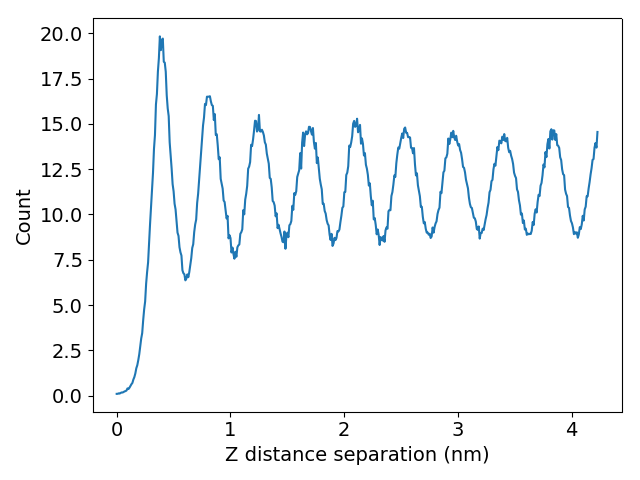
\includegraphics[width=\textwidth]{zdf5layered.png}
		\caption{}\label{fig:zdf_layered}
	\end{subfigure}
	\begin{subfigure}{0.45\textwidth}
		\centering
		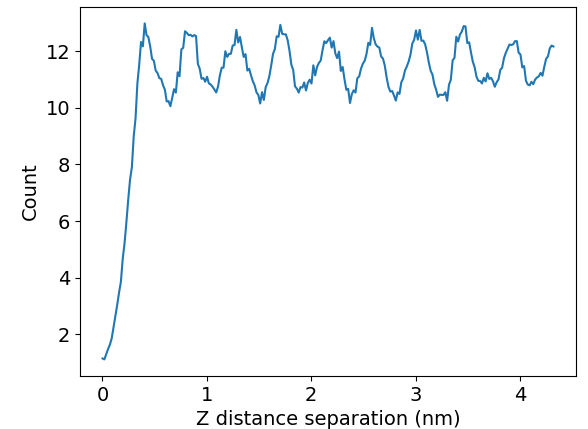
\includegraphics[width=\textwidth]{zdf5offset.png}
		\caption{}\label{fig:zdf_offset}
	\end{subfigure}
	\caption{Pair distribution functions of aromatic carbons for the
	(a) 5 monomer per layer, sandwiched and (b) 5 monomer per layer, 
	parallel displaced configurations. 
        %MRS: added some info.
        Clear periodic maxima in the $z$ probability density indicate
        % Spikes in the distribution mark
	distinct layers. The magnitude of the spikes with respect to the 
	average suggest that the 5 monomer per layer, sandwiched configuration
	possesses a higher degree of layer partitioning.}\label{fig:zdf}
  \end{figure}

  Experimental WAXS measurements encode all remaining structural details. 
  %MRS: also encodes the pore spacing
  %BJC: I'm not exactly sure where to place this paragraph. Maybe it can go in methods?
  \begin{itemize}
  	\item There are five major features present in the 2D experimental 
	pattern which our model intends to reproduce (Figure~\ref{fig:WAXS}).
	\item The first is located at qz = 1.7 \angstrom \textsuperscript{-1},
	corresponding to a real spacing of 3.7 \angstrom. The reflection is 
	attributed to pi-pi stacking between aromatic rings in the direction
	perpendicular to the membrane plane, or z-axis. For simplicity, this 
	reflection will be referred to as R-pi.
        %MRS: why R in R-pi? for reflection?
	\item A weak intensity line is located at exactly half the qz value of
	R-pi (qz = 0.85 \angstrom \textsuperscript{-1}), corresponding to a 
        %MRS: or could use \angstrom$^-1$ instead of \textsuperscript{-1} 
	real space periodic spacing of 7.4 \angstrom. This reflection has been 
	interpreted  as 2\textsubscript{1} helical ordering of aromatic rings 
	along the z axis meaning if the positions of the aromatic rings can
	be traced by a helix, then for each turn in the helix, there should be
	two aromatic rings. For this reason it will be referred to as R-helix.
	\item A third major reflection is marked by a low intensity ring located
	at r = 1.4 \angstrom \textsuperscript{-1}. The real space separation 
	corresponds to 4.5 \angstrom which is characteristic of the average 
	spacing between packed alkane chains. This reflection will be called R-alkanes.
	\item Within R-alkanes, are four spots of higher intensity which 
	will be called R-spots. All are located $\approx 40$ degrees from the qz axis
	in their respective quadrants. In many liquid crystal systems this can be
	explained by the tilt angle of the alkane chains with respect to the xy plane. % BJC: Reference
	\item The final major reflections correspond to the spacing and symmetry of 
	the d\textsubscript{100} plane which can be related to the distance between
	pores. The feature, which will be called R-pores, is characterized by dots 
	along qz = 0. The spacing between dots is indicative of the hexagonal 
	symmetry of the packed pores. It is easiest to interpret the data by 
	radially integrating the 2D data to get a 1D curve which is shown in Figure~\ref{fig:SAXS}.
  \end{itemize}

  \begin{figure}[!ht]
	\centering
	\begin{subfigure}[t]{0.47\linewidth}
		\centering
		\raisebox{.2\textwidth}{%
		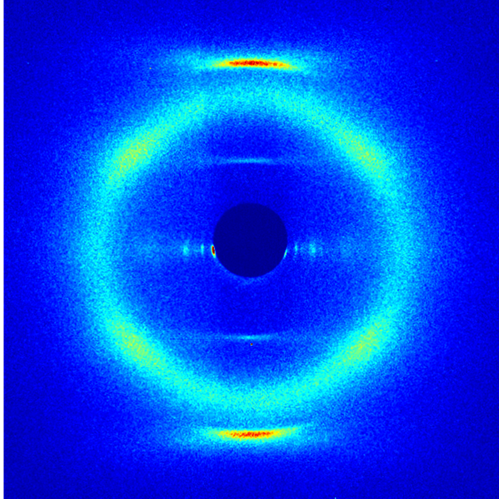
\includegraphics[width=\linewidth]{WAXS_soft_confined.png}
		}
		\caption{}\label{fig:WAXS}
	\end{subfigure}
	\begin{subfigure}[t]{0.43\linewidth}
		\centering
	%	\vspace{12mm}
		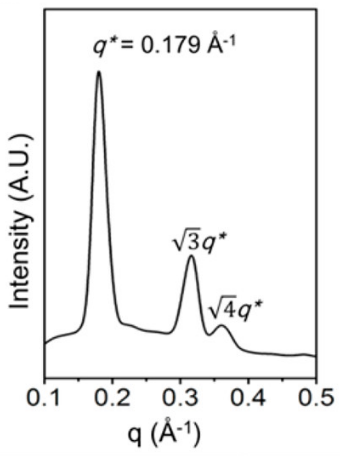
\includegraphics[width=\linewidth]{SAXS.png}
		\caption{}\label{fig:SAXS}
	\end{subfigure}
	\caption{(a) 2D wide angle X-ray scattering gives details about repeating
	features less than 1 nanometer apart. (b) 1D small angle X-ray scattering 
	indicates hexagonal packing of pores as well as the spacing between pores.}\label{fig:SWAXS}
        %MRS: maybe compare the 2D and 1D from simulation here as well?  Need to state the above figure is from another paper (I think at least the 1D is?)
  \end{figure}
  
  The initial distance between layers can influence the approach towards
  equilibrium. 
  \begin{itemize}
  	\item Equilibrated systems built according to the 3.7 \angstrom 
	layer spacing implied by R-pi are characterized by a defined, cylindrical and
	open pore structure.
	\item Aromatic rings are arranged in a helical conformation.%BJC: could potentially support with a figure. Mentioning the helical arrangmentment might makes things confusing though
        %MRS: 'basin' is not that common a term, and also only makes sense if one explicitly states what 
        %MRS: the basin is with respect to. 
        We will refer to this large set of configurations, with an open helical pore, as Basin A (Figure~\ref{fig:abasin}).
        %\item We will refer to this system as
        %MRS: maybe Basin O and Basin C for open and closed?
	\item Simulations of systems built with layers stacked greater than 4 
	\angstrom apart results in a pore structure characterized by high radial 
	disorder, while still maintaining partitioning between hydrophobic and 
	hydrophilic regions.
        %MRS: see above for clarifying ``basins''.
	\item This will be called Basin B (Figure~\ref{fig:bbasin}).
        %MRS: I don't think enough information has been presented to the reader yet for this to be 'apparent'.
	\item It is apparent that this LLC membrane may exist in at least two metastable states.
	\item The distinct difference in pore structure exhibited by each phase will 
	likely lead to different transport mechanisms.
	\item Understanding which phase exists experimentally is necessary in order
	to appropriately study the system.  %MRS: remind people why.
  \end{itemize}
  
  \begin{figure}[!ht]
        \centering
        \begin{subfigure}[b]{0.475\textwidth}
                \centering
                \includegraphics[width=\textwidth]{280K_tramp_close.png}
                \caption{}\label{fig:abasin}
        \end{subfigure}
        \begin{subfigure}[b]{0.475\textwidth}
                \centering
                \includegraphics[width=\textwidth]{340K_tramp_close.png}
                \caption{}\label{fig:bbasin}
        \end{subfigure}
	\caption{From a qualitative standpoint, Basin A (a) is characterized by a
	hollow cylindrical pore while pores in Basin B (b) are characterized by a
	higher degree of radial disorder}\label{fig:basins}
  \end{figure}

  %MRS: by this point, it's not clear that the directions at the
  %beginning have clearly laid out what is being done. You want all of
  %the logic you are going to use to be laid out by the introduction,
  %so that only the results are left to reveal.  Fit what you are doing 
  %in the logic pattern you lay out (which may sometimes require adjusting the logic a bit)

  We varied the relative interlayer orientation between sandwiched and 
  parallel-displaced based on our knowledge of the stability of the two
  pi-stacking modes.
  \begin{itemize}
  	\item We generated simulated X-ray diffraction patterns from the highly
	restrained initial configurations created during equilibration
	\item The patterns establish a difference between the two stacking 
	modes (Figure~\ref{fig:XRDrestrained}).
	\item In each pattern, R-alkanes is present at a distance of $\approx
	1.5$ \angstrom \textsuperscript{-1} (4.2 \angstrom in real space).
  	\item R-pi is also present in each pattern, although it appears to 
	intersect R-alkanes because the spacing between aromatic rings is 
	similar to the alkane chain packing.
        %MRS: for above, may need to clarify that this is in simulation, which is different than experiment.
	\item The difference in aromatic ring spacing between experiment and
	simulation is likely a result of the inability of GAFF to properly handle
	aromatic interactions. %MRS: provide citations, some mechanistic reasoning.
	\item The sandwiched configuration shows R-spots in the expected location.
	\item A faint reflection is present in the location of R-helix %BJC: but it fades upon further simulation.
	\item The parallel displaced configuration contains two lines of high 
	intensity with maximum intensity occurring where they intersect the alkane
	chain region due to constructive interference between the two features.
	\item The lines are located where one would expect to see R-helix and, 
	perhaps coincidentally, the intersection with R-alkanes occurs where one 
	would expect to see R-spots.
	%BJC: might save the following sentence for equilibrium trajectories
	\item As the simulation is progressed, the full line begins to fade 
	(Figure~\ref{fig:XRDsim}). Most significantly, the line is no longer present
	where R-helix exists.
  \end{itemize}

  \begin{figure}[!ht]
	\centering
	\begin{subfigure}{0.475\textwidth}
		\hspace{-1.2cm}
		\centering
		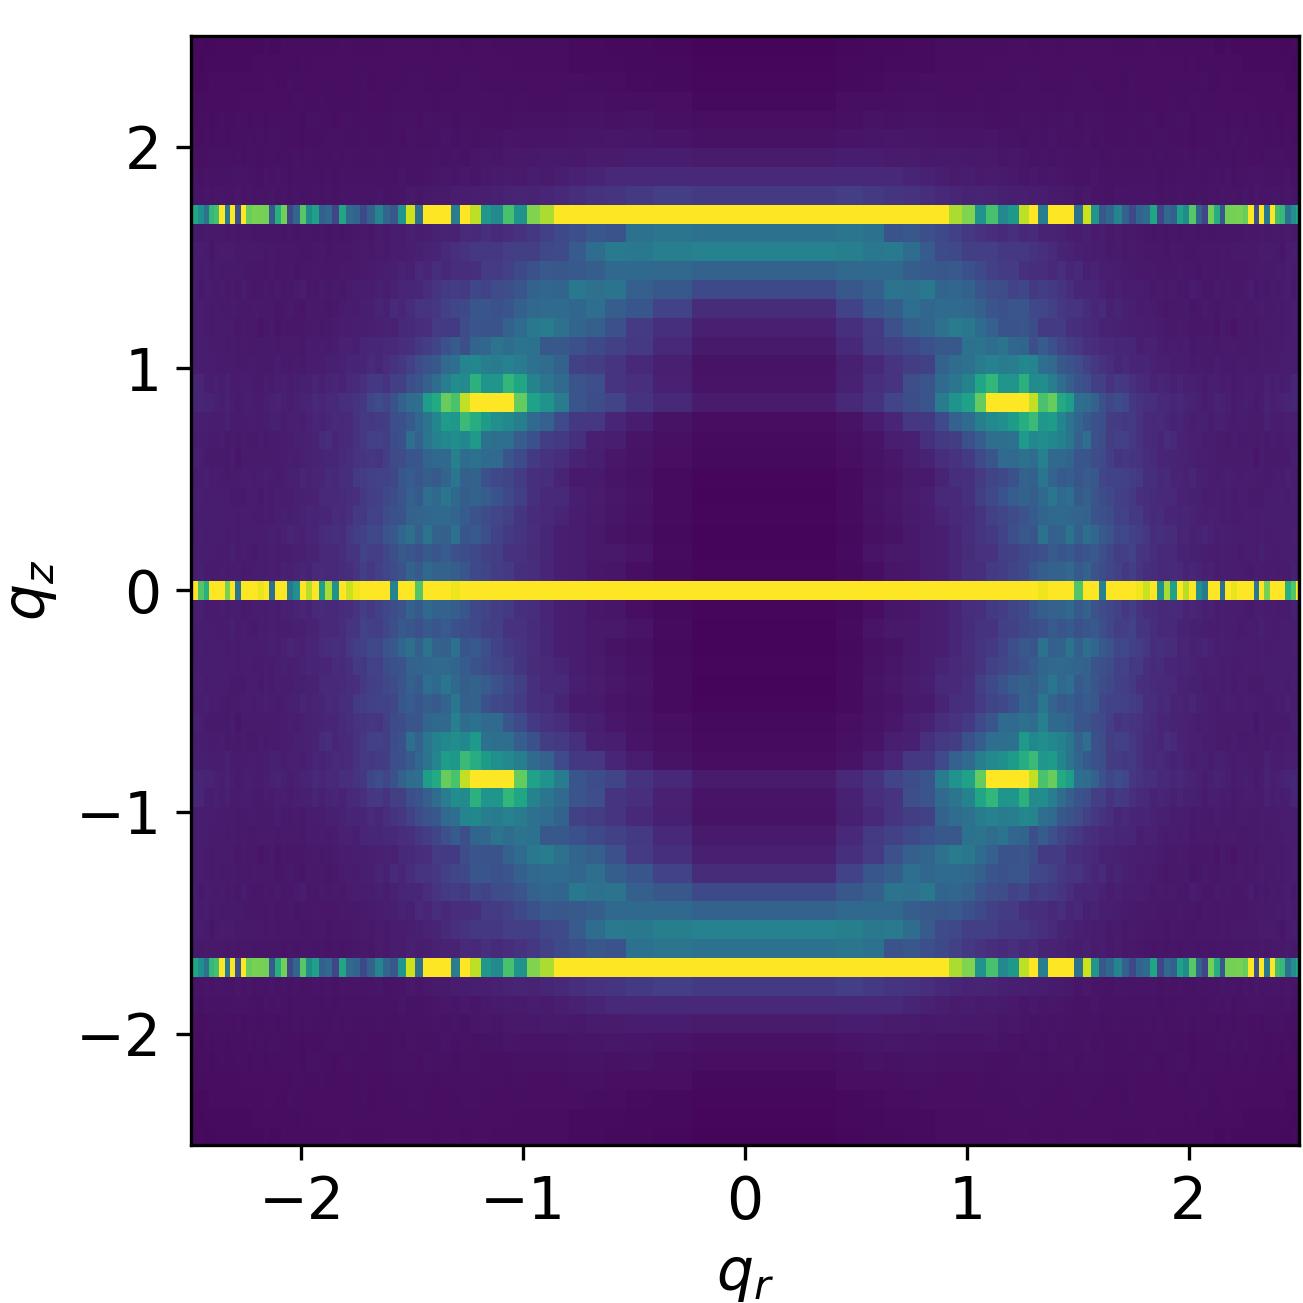
\includegraphics[width=\textwidth,valign=t]{rzlayeredrestrained.png}
		\caption{}\label{fig:rzplayeredrestrained}
	\end{subfigure}
	\begin{subfigure}{0.475\textwidth}
		\hspace{-1.2cm}
		\centering
		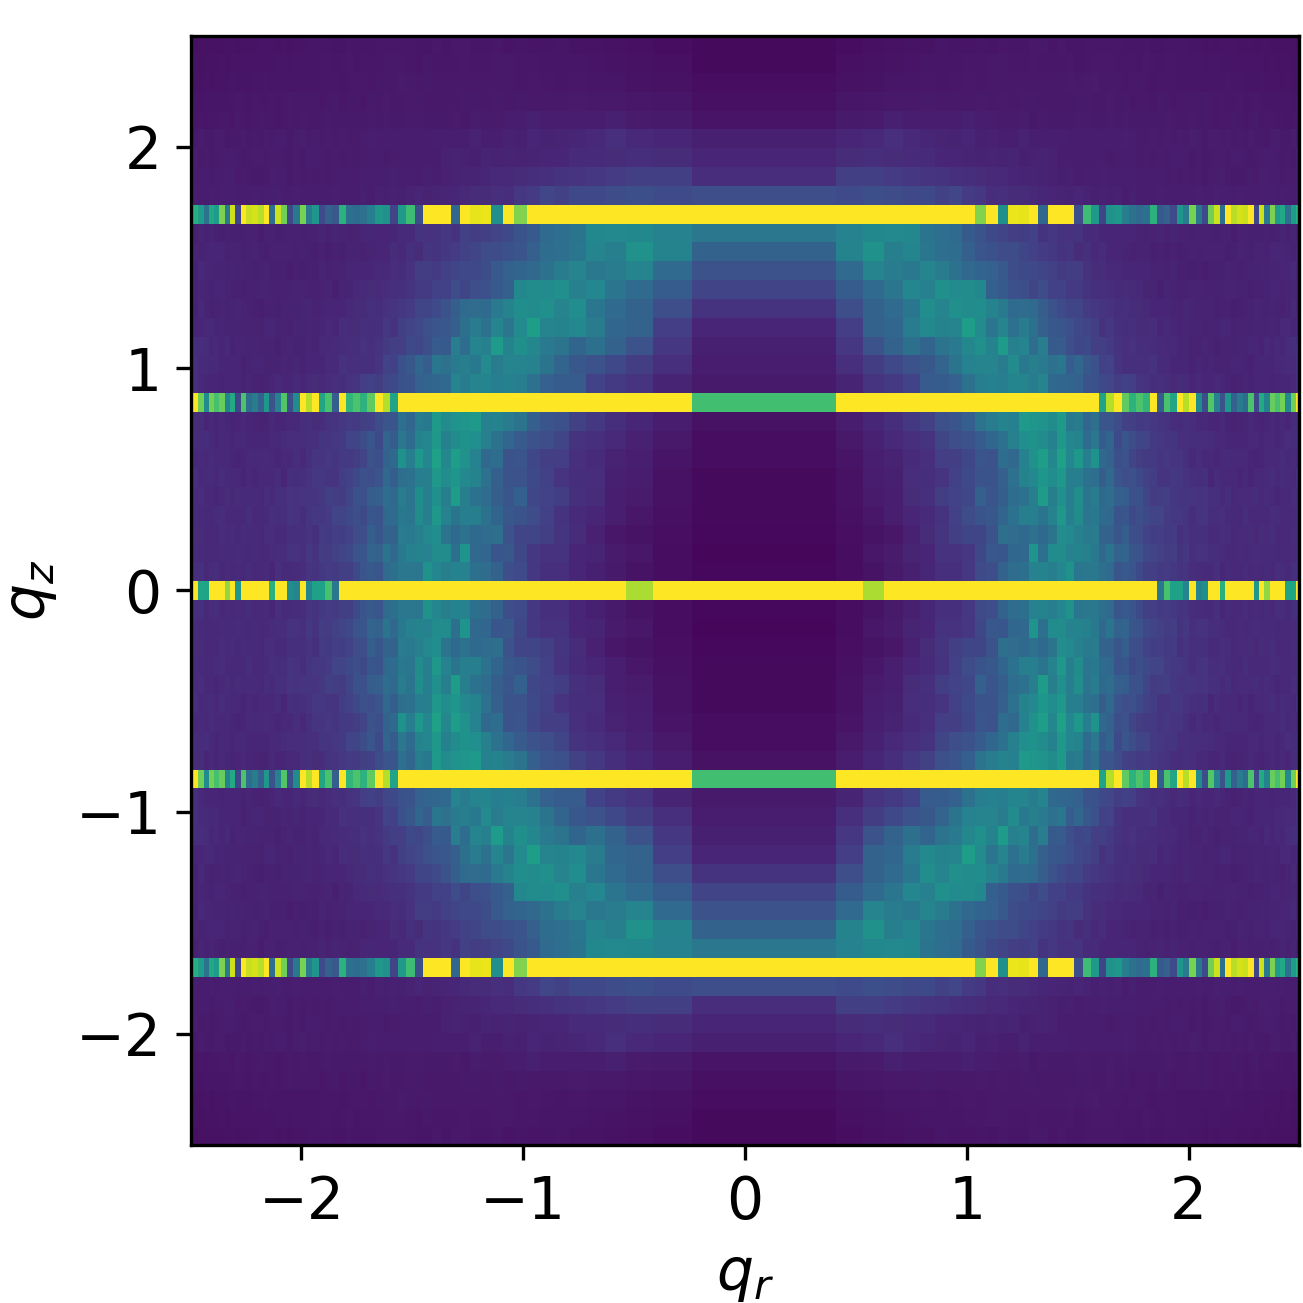
\includegraphics[width=\textwidth,valign=t]{rzoffsetrestrained.png}
		\caption{}\label{fig:rzoffsetrestrained}
	\end{subfigure}
	\caption{(a) Simulated X-ray diffraction of a sandwiched configuration
	with restraints placed on aromatic carbons shows all major features
	present in experimental WAXS. Near solid lines at constant z are a result of 
	the highly ordered aromatic rings. (b) Simulated X-ray diffraction of a similarly
	restrained parallel displaced configuration may also contain all
	major experimental WAXS features. One can argue that R-spots is not present
	but it is difficult to distinguish because of its intersection with the solid
	R-helix line. 
        %MRS: Longer simulations are necessary to determine which structure
	is the best match to experiment
        %MRS: we probably want to avoid saying this (above) if we can.
}\label{fig:XRDrestrained}
  \end{figure}

  %MRS: one thought: maybe organize it a different way -- it's not the disordered (and go through the anlysis there), and then separately show that it's more likely the sandwich.  Something to think about.
  %MRS: anyway, this is the key part of the paper, so clarity and organization important.
  %MRS: make sure the figures are comparable.  Could someone look at the figures, and see immediately what you are explaining -- for example, experiment and fully equilibrated disordered, sandwich and parallel displaced all in a row?
  Full comparison of experimental 2D WAXS with simulated X-ray diffraction
  patterns produced from equilibrated MD trajectories shows the most consistency
  with the sandwiched configuration in Basin A.
  \begin{itemize}
  	\item Systems were built in both the parallel displaced and sandwiched 
	configurations with an intial layer spacing of 3.7 \angstrom.
	\item A third system was created by stacking layers in the sandwiched 
	configuration 5 \angstrom apart in order to guide it towards Basin B.
	% BJC: I've done an additional offset disordered system which goes to Basin B but I think that will confuse the point
	\item For ease of reference, the third system will be referred to as the disordered system. 
%BJC: omit and call it basin B
%MRS or just be consistent from the beginning.  Or call Basins O and D          
	\item The three systems were equilibrated according to our procedure with
	NPT simulations of greater than 400 ns.
	\item Simulated diffration patterns were generated using portions of the
	trajectory after equilibration.
%MRS: something like ``we assume the simulation has equilibrated when the distance . . . ``        
	\item Equilibration was detected when the distance between pores and the 
	membrane thickness stopped changing.
	\item Simulated diffraction patterns for all three structures are shown in 
	Figure ~\ref{fig:XRDsim}. 
	%BJC: maybe break into a separate paragraph starting here
	\item The equilibrated parallel displaced structure exhibits R-alkanes and
	R-pores in the expected locations. 
	\item Due to low resolution, making out the individual spots of R-pores is
	challenging and can be validated upon full spherical integration of the 3D 
	structure factor. However, the same information can be extracted by measuring 
	the pore spacing as described earlier.
	\item R-pi is also present, intersecting R-alkanes at a lower q value than
	in experiment. The rings prefer to stack $\approx 4.1 \angstrom$ apart as 
	opposed to 3.7 \angstrom.
	\item R-helix and R-spots are also both missing.
	\item The line which intersected both of these features in the restrained 
	simulations faded upon equilibration which suggests that monomers in the 
	parallel-displaced configuration may not give rise to the experimental WAXS 
	pattern seen.
	\item Simulated XRD of the sandwiched configuration contains all features 
	except for R-helix.
	\item Most notably, R-spots appears in the expected location, which suggests 
	that there is something intrinsic to the sandwiched packing that gives rise 
	to such features. 
	\item Finally, the disordered structure exhibits R-alkanes and R-pores but 
	R-helix, R-pi and R-spots are not present.
  \end{itemize}
  
  \begin{figure}[!ht]
	\centering
	\begin{subfigure}{0.31\textwidth}
		\centering
		\hspace{-0.9cm}
		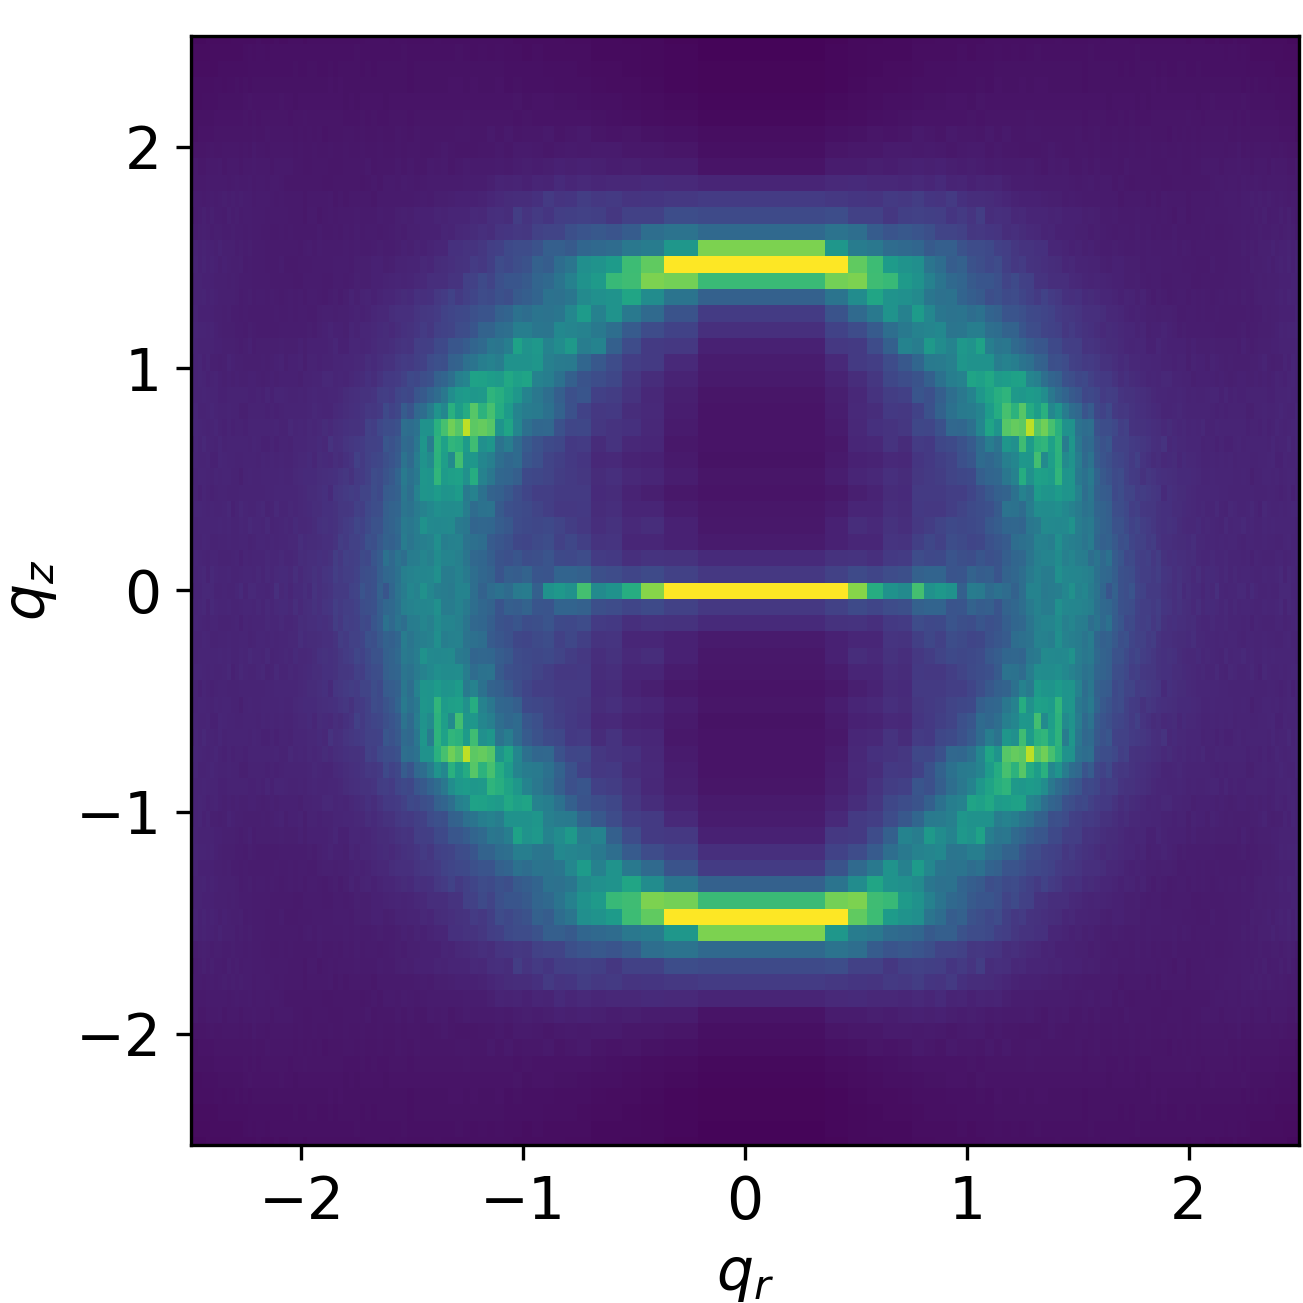
\includegraphics[width=\textwidth]{sandwich_rzplot.png}
		\caption{}\label{fig:sandwich_rzplot}
	\end{subfigure}
	\begin{subfigure}{0.31\textwidth}
		\centering
		\hspace{-0.9cm}
		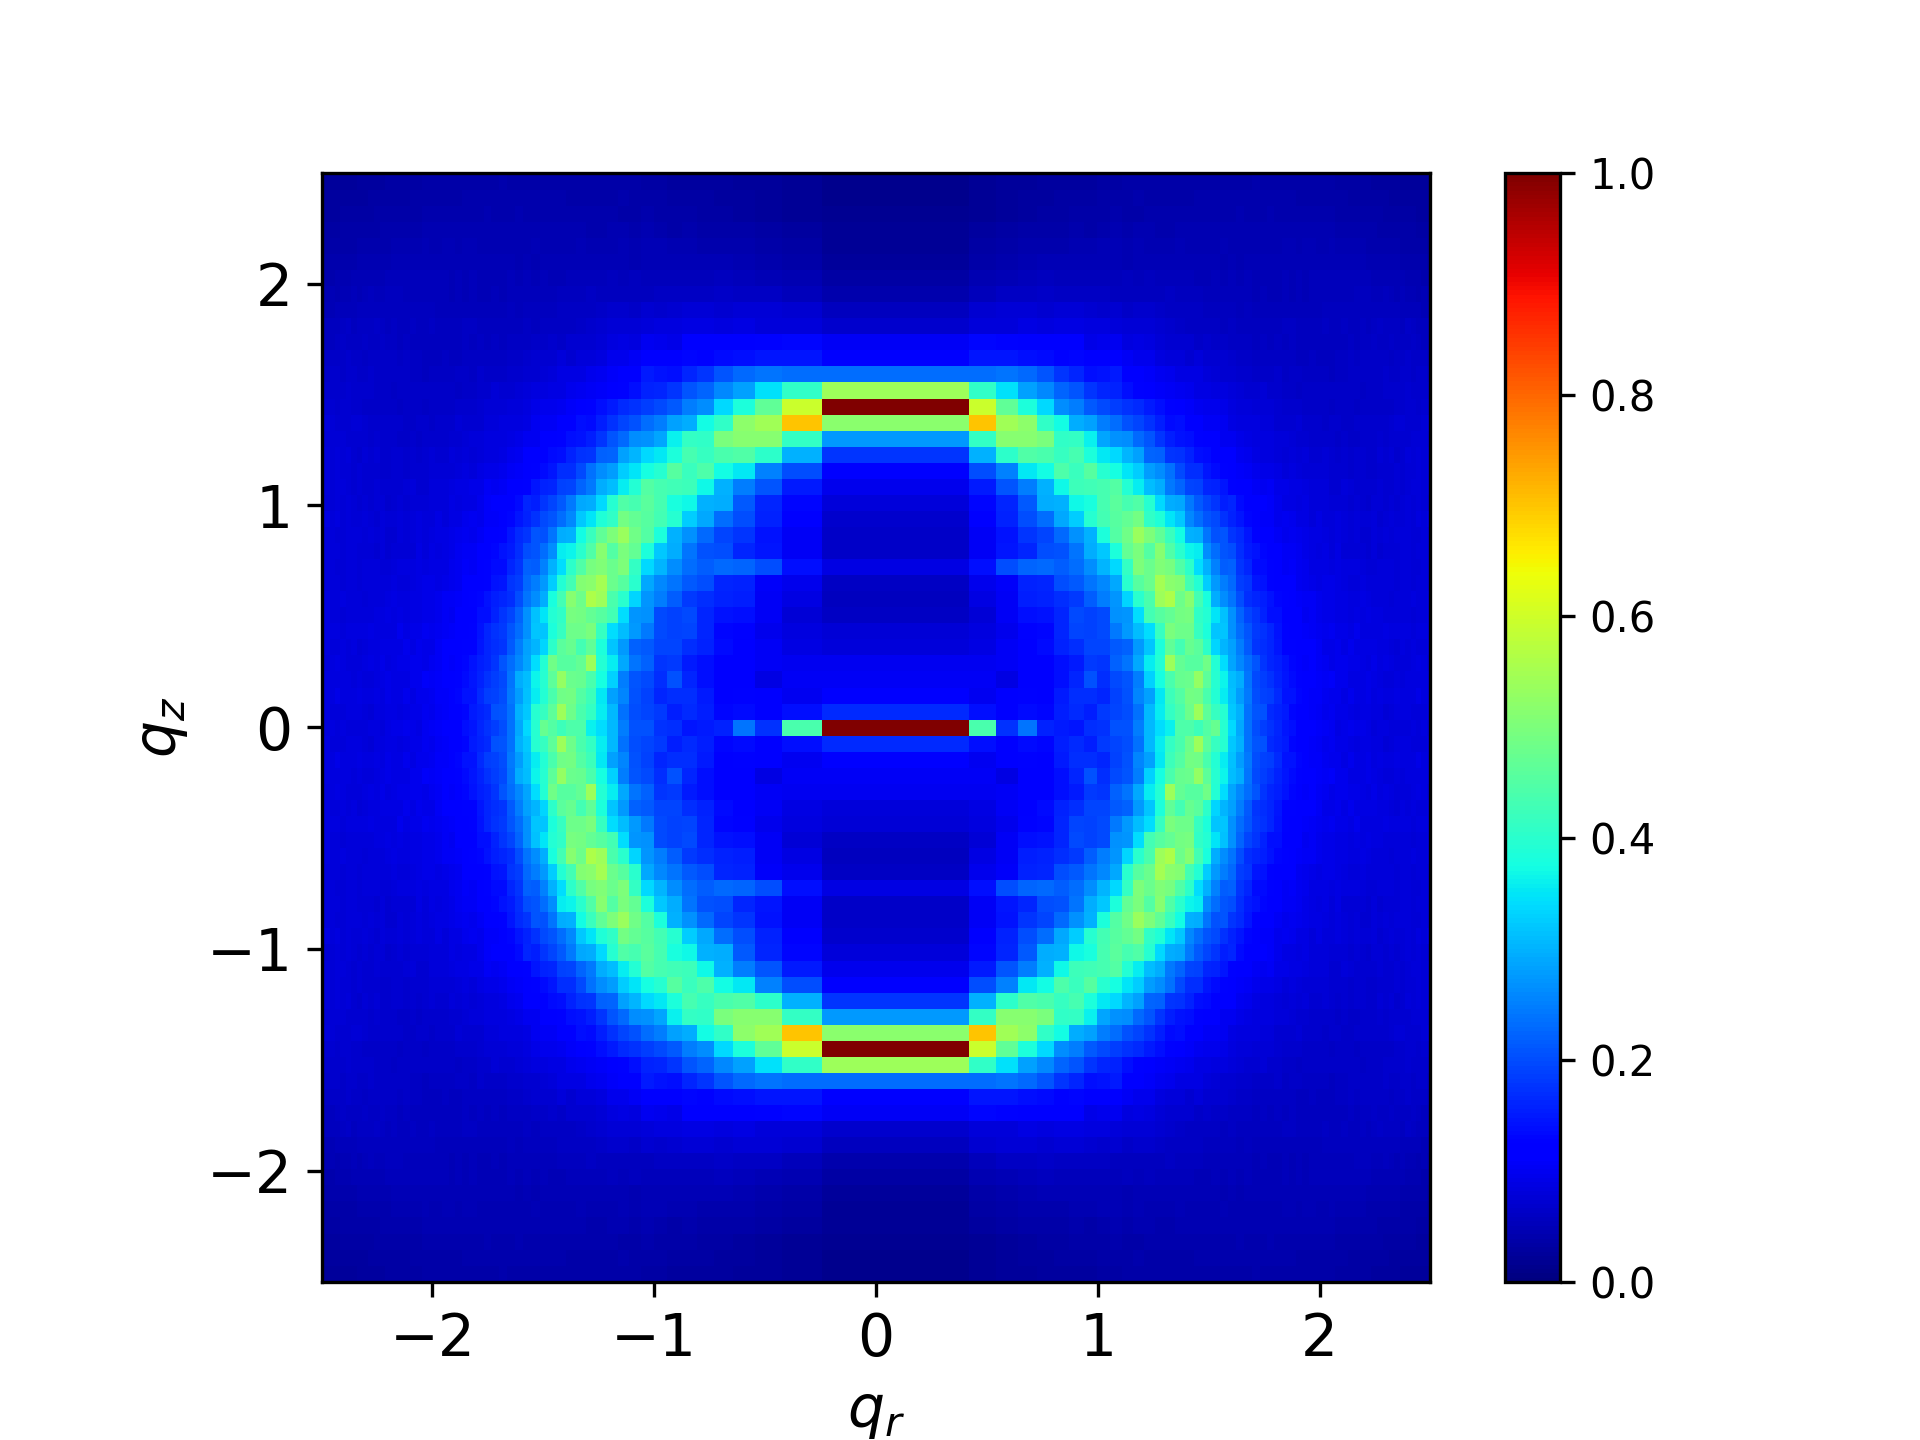
\includegraphics[width=\textwidth]{offset_rzplot.png}
		\caption{}\label{fig:offsetrzplot}
	\end{subfigure}
	\begin{subfigure}{0.31\textwidth}
		\centering
		\hspace{-0.9cm}
		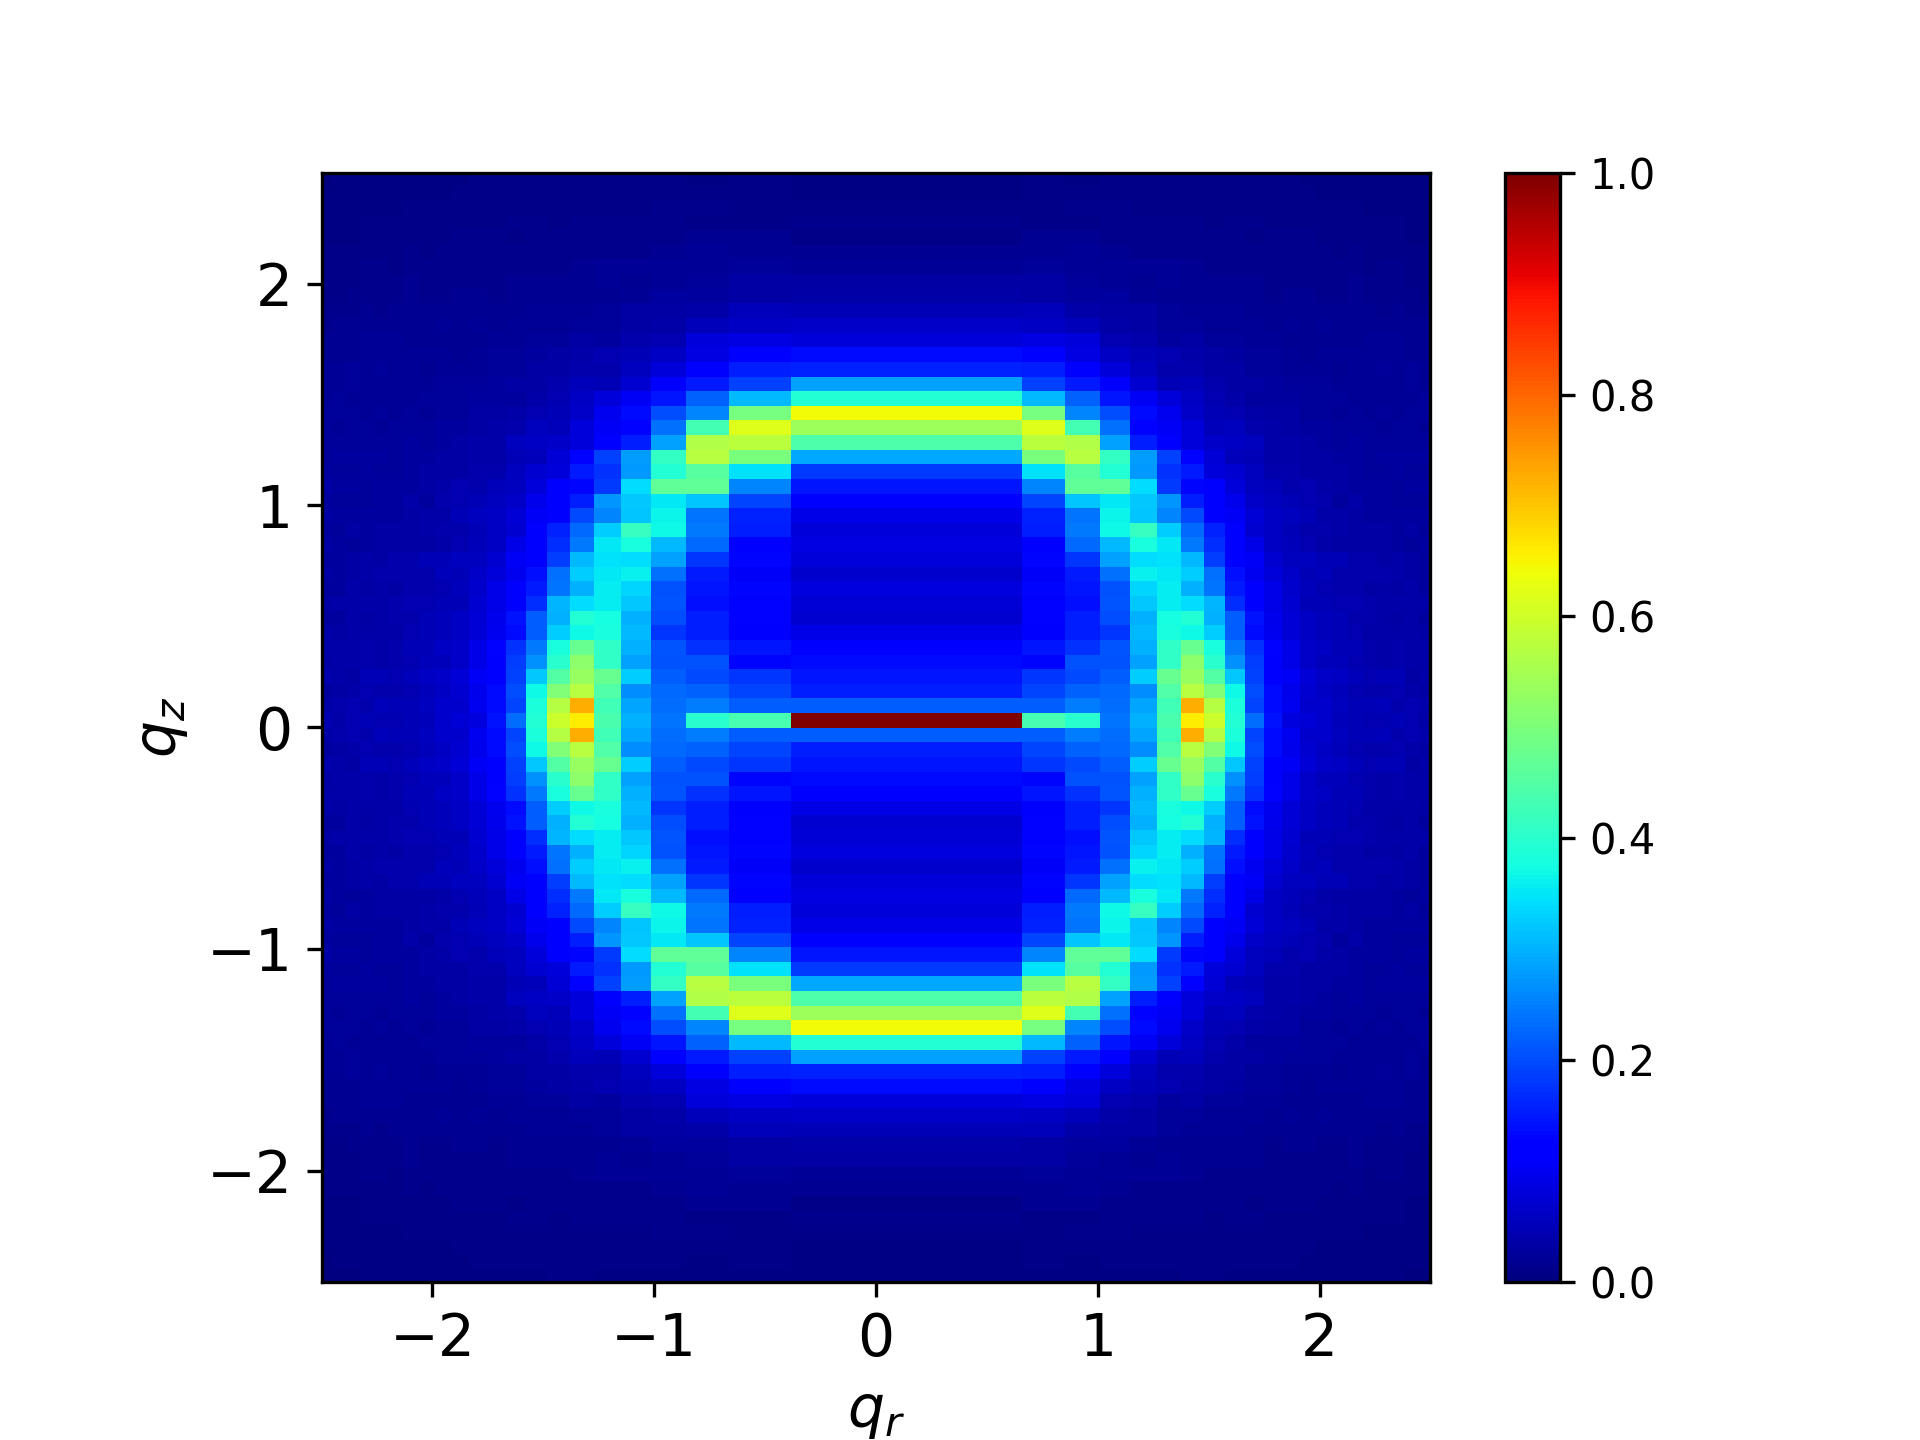
\includegraphics[width=\textwidth]{disorder_rzplot.png}
		\caption{}\label{fig:disorder_rzplot.png}
	\end{subfigure}
	\caption{(a) All major features except R-helix are present in
	XRD patterns resulting from an equilibrated sandwiched configuration 
	in Basin A. R-pi intersescts R-alkanes. R-helix faded during equilbration.
	(b) All major features execpt R-spots are present in XRD patterns 
	resulting from an equilibrated parallel displaced configuration in Basin A.
	R-helix exists faintly in the expected location. (c) R-pores and R-alkanes
	are the only major features present in XRD patterns resulting from an 
	equilibrated disordered phase}\label{fig:XRDsim}
  \end{figure}

  \begin{wrapfigure}{R}{0.4\textwidth}
        \centering
        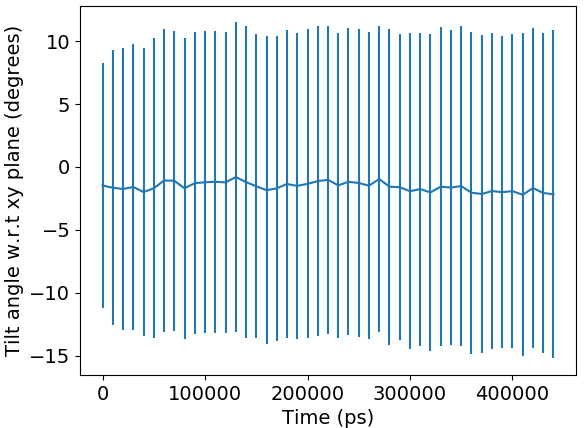
\includegraphics[width=0.4\textwidth]{tilt.png}
        \caption{The average angle between alkane chains and the xy plane is nearly zero degrees}\label{fig:tilt}
        %MRS: probably could just report this in text, put figure in supporting.
  \end{wrapfigure}
  
  The spots that appear in the simulated XRD pattern of the sandwiched
  conformation are a result of the way alkane tails pack together.
  \begin{itemize}
  	\item Previously, the spots in the diffraction pattern had been explained 
	as the product of tilted alkane chains.
	\item We measured the tilt angle of the alkane chains and showed that our 
	system equilibrates to an average tilt angle close to zero degrees (Figure~\ref{fig:tilt}). 
	\item To understand the origin of the spots, we determined which atoms gave rise to the feature.
	\item By removing atoms from the trajectory and simulating a diffraction 
	pattern, we were able to isolate the cause of the spots to the tails (Figure~\ref{fig:tails_rzplot}).
	\item Since the tails are mostly flat, we plotted the centroids of the 
	tails and measured the angle between each centroid and its nearest neighbors
	with respect to the plane of the membrane (Figure~\ref{fig:centroids}).
	\item The distribution of these angles is consistent with the location of 
	the spots (Figure~\ref{fig:angle_distribution}).
	\item We reason that monomer tails stacked closely in the sandwiched conformation
	are forced to splay apart and pack in between in each other which creates a
	nearly hexagonal array of packed tails. 
        %MRS: hmm.  and this doens't happen in parallel displaced? I thought it did.
        %thought it did before. Would be good to explore the equivalent of figure 9 to this, because that comparison would make it clearer what the structural reason is for the R-spots.
  \end{itemize}
  
  \begin{figure}[!ht]
	\centering
	\begin{subfigure}{0.45\textwidth}
		\centering
		\hspace{-1cm}
		\vspace{1cm}
		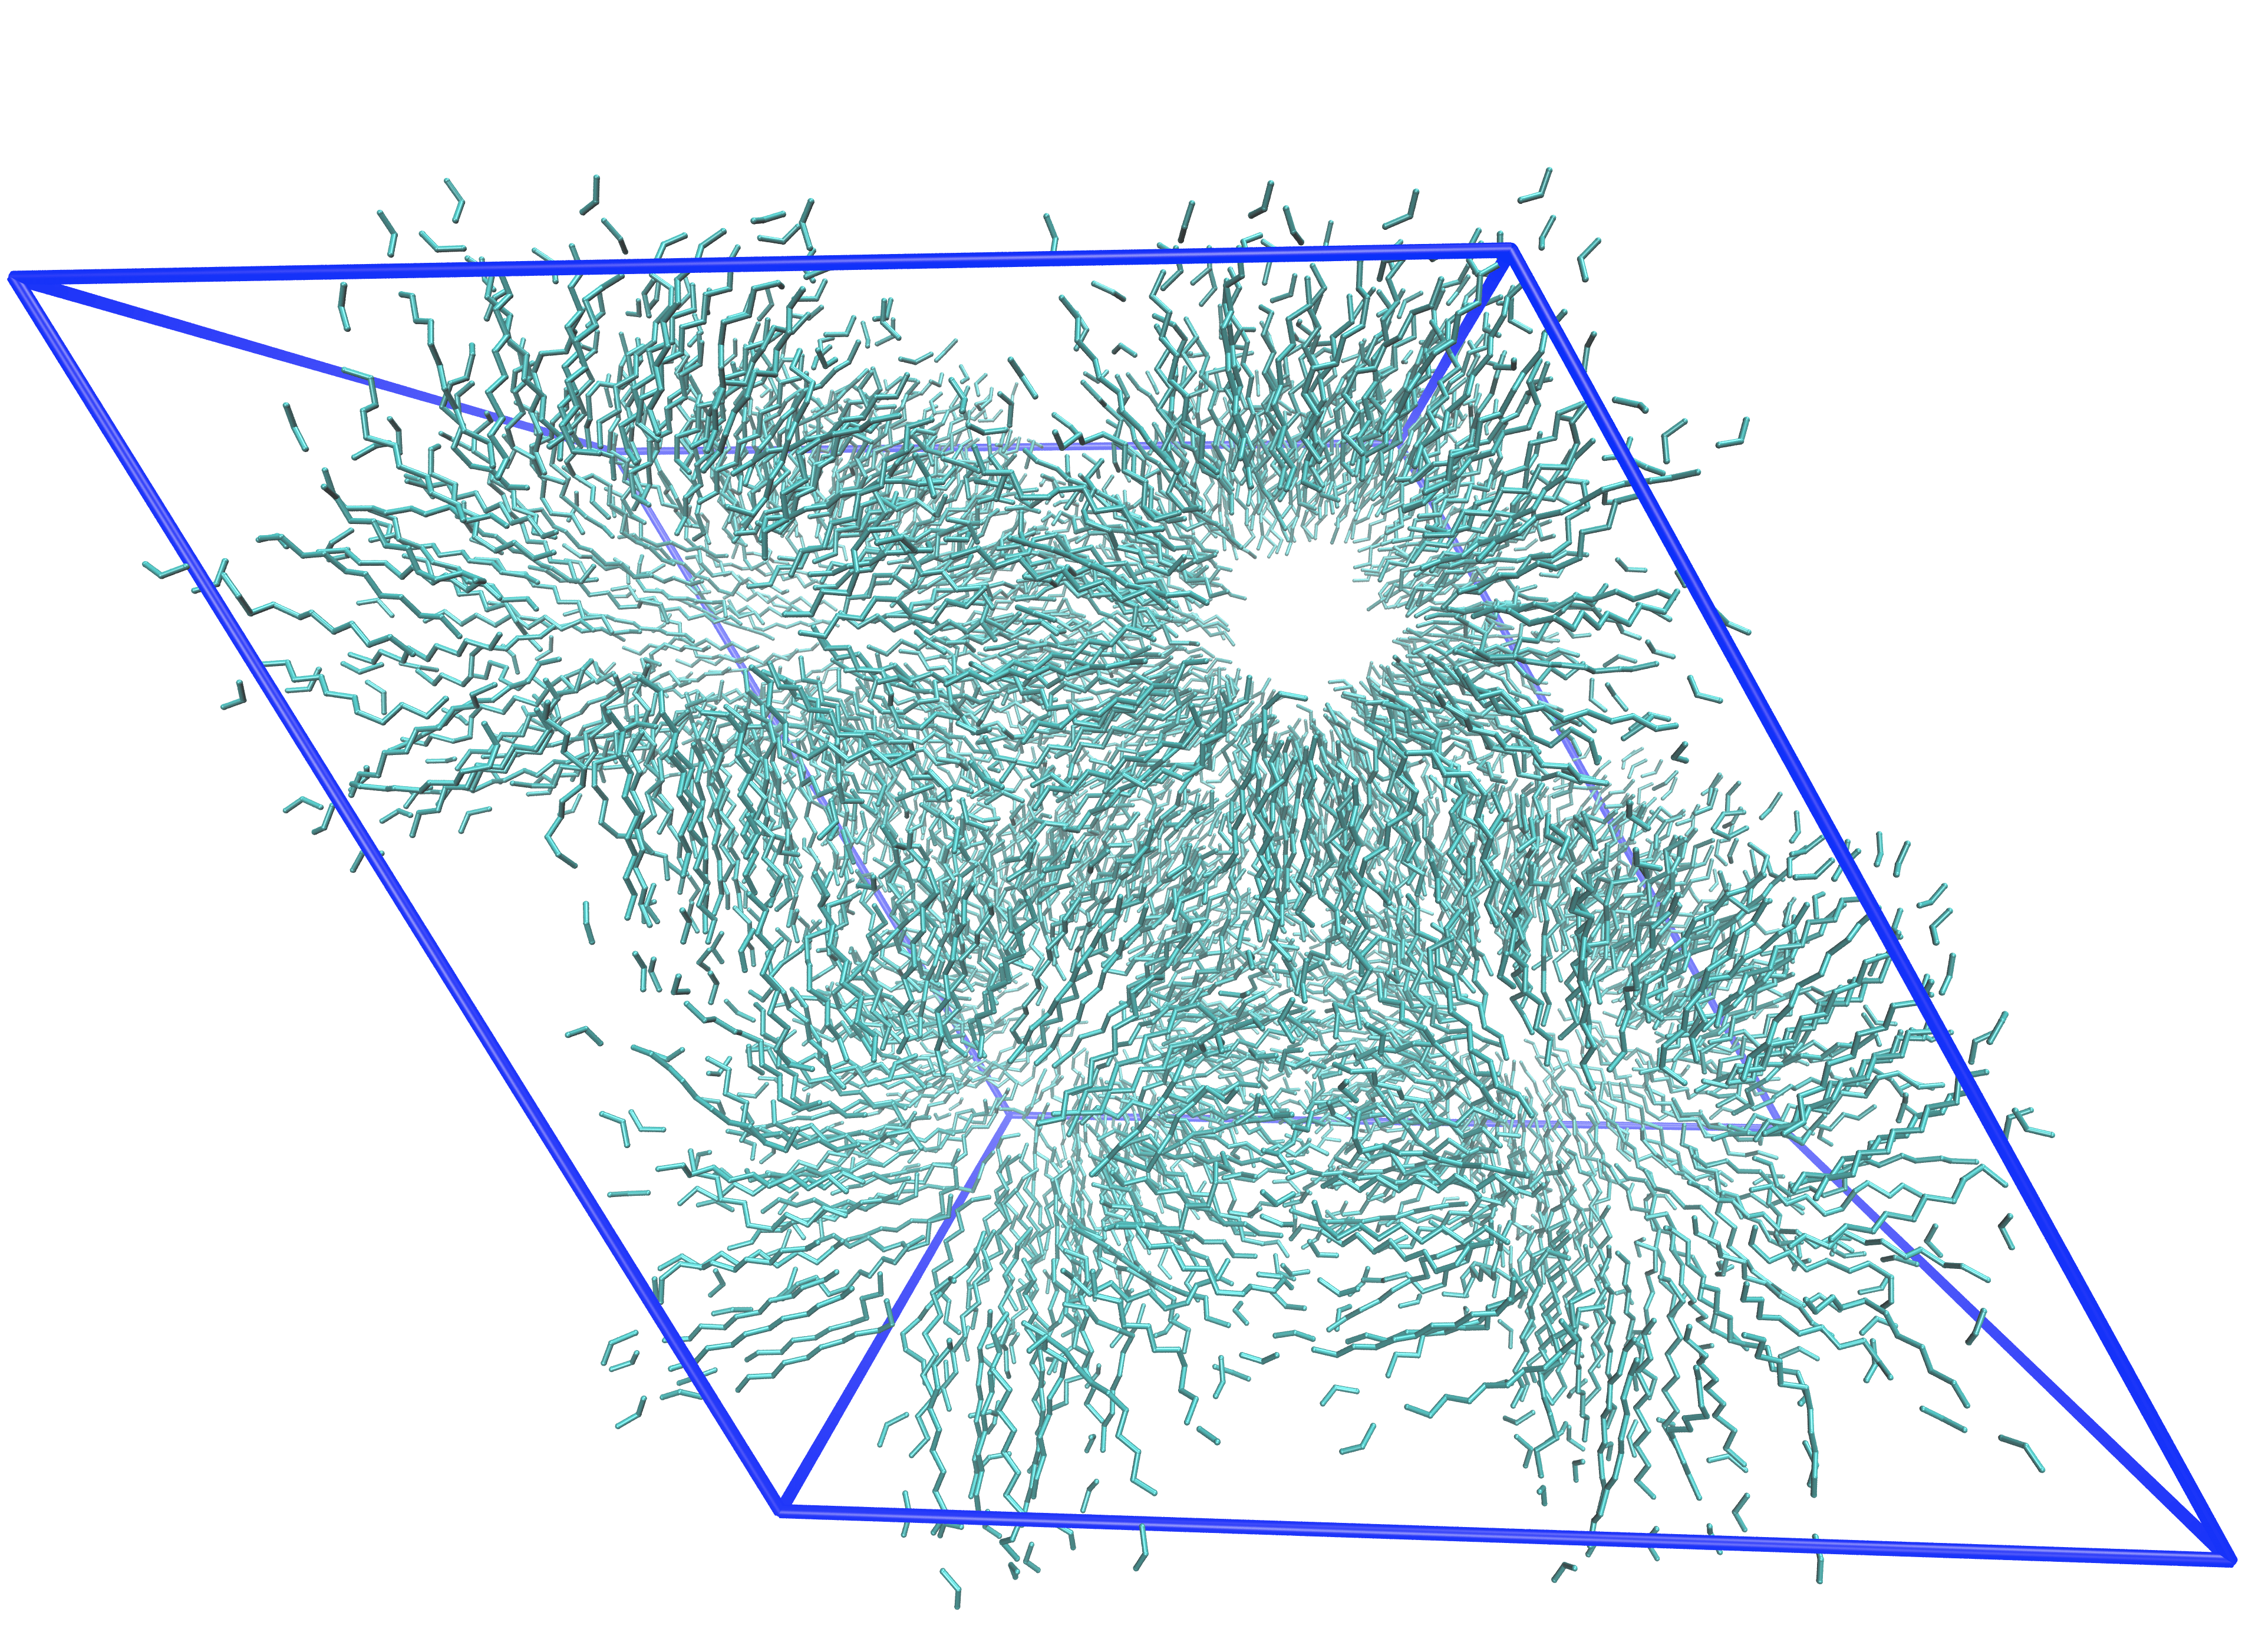
\includegraphics[width=\textwidth,scale=2]{tails_topview.png}
		\caption{}\label{fig:tails_topview}
	\end{subfigure}
	\begin{subfigure}{0.45\textwidth}
		\centering
		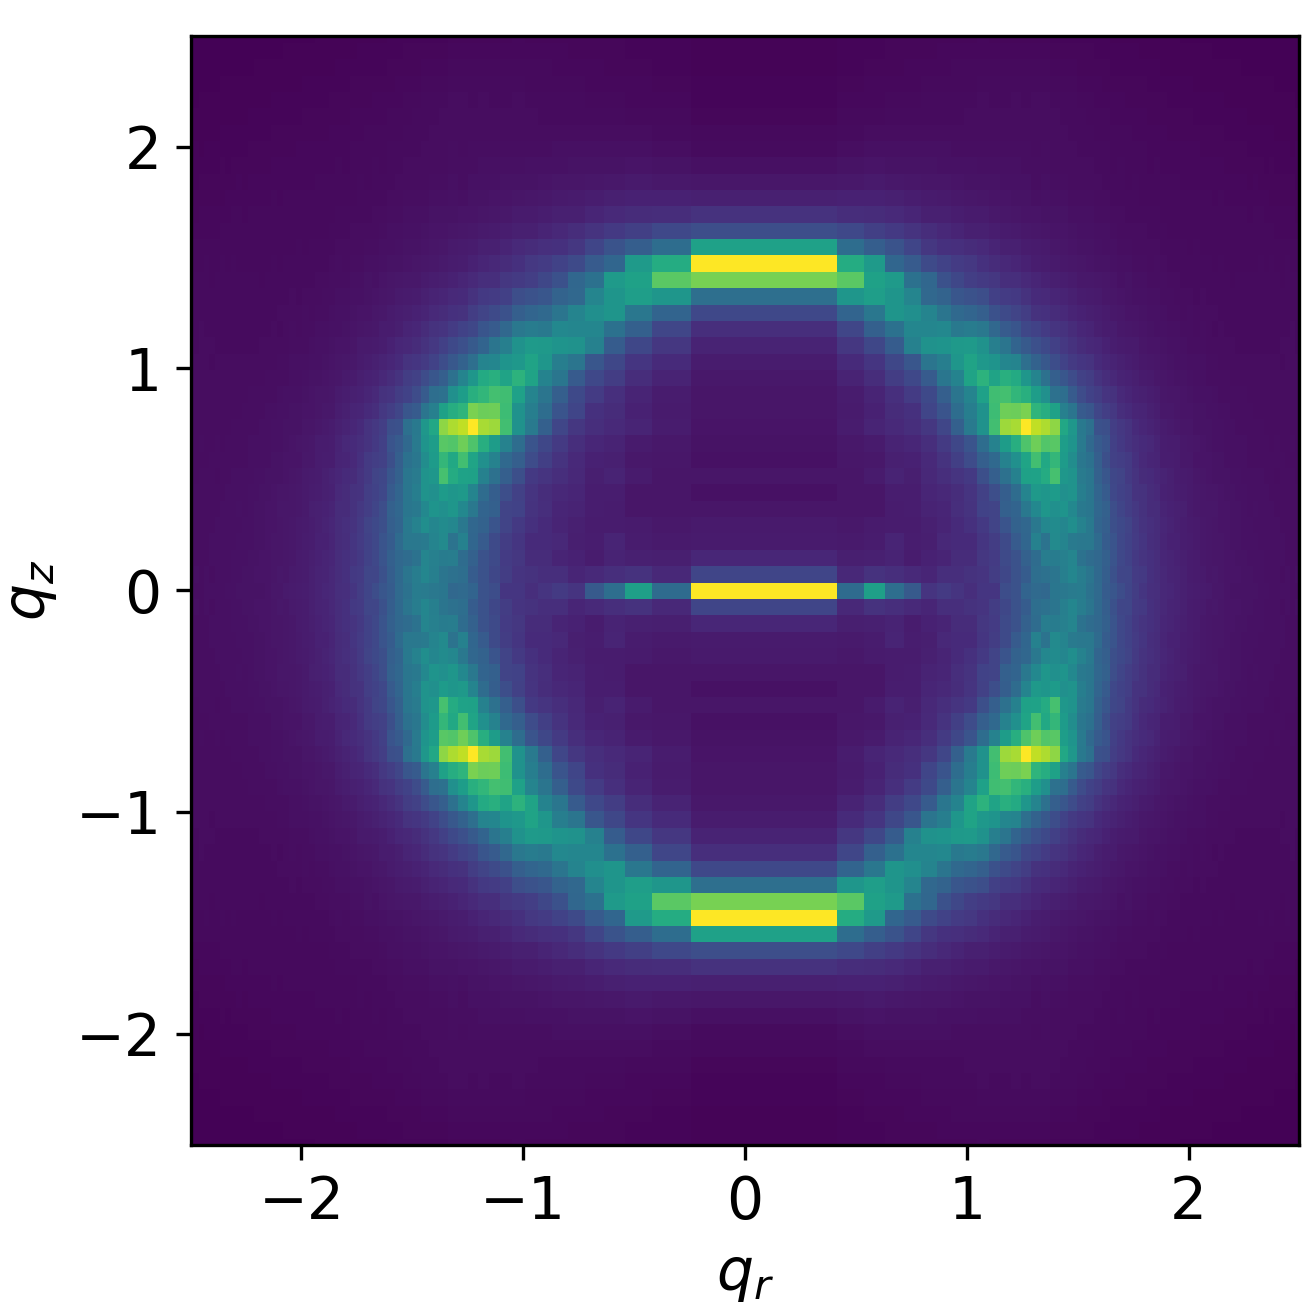
\includegraphics[width=\textwidth]{tails_rzplot.png}
		\caption{}\label{fig:tails_rzplot}
	\end{subfigure}
	\begin{subfigure}{0.45\textwidth}
		\centering
		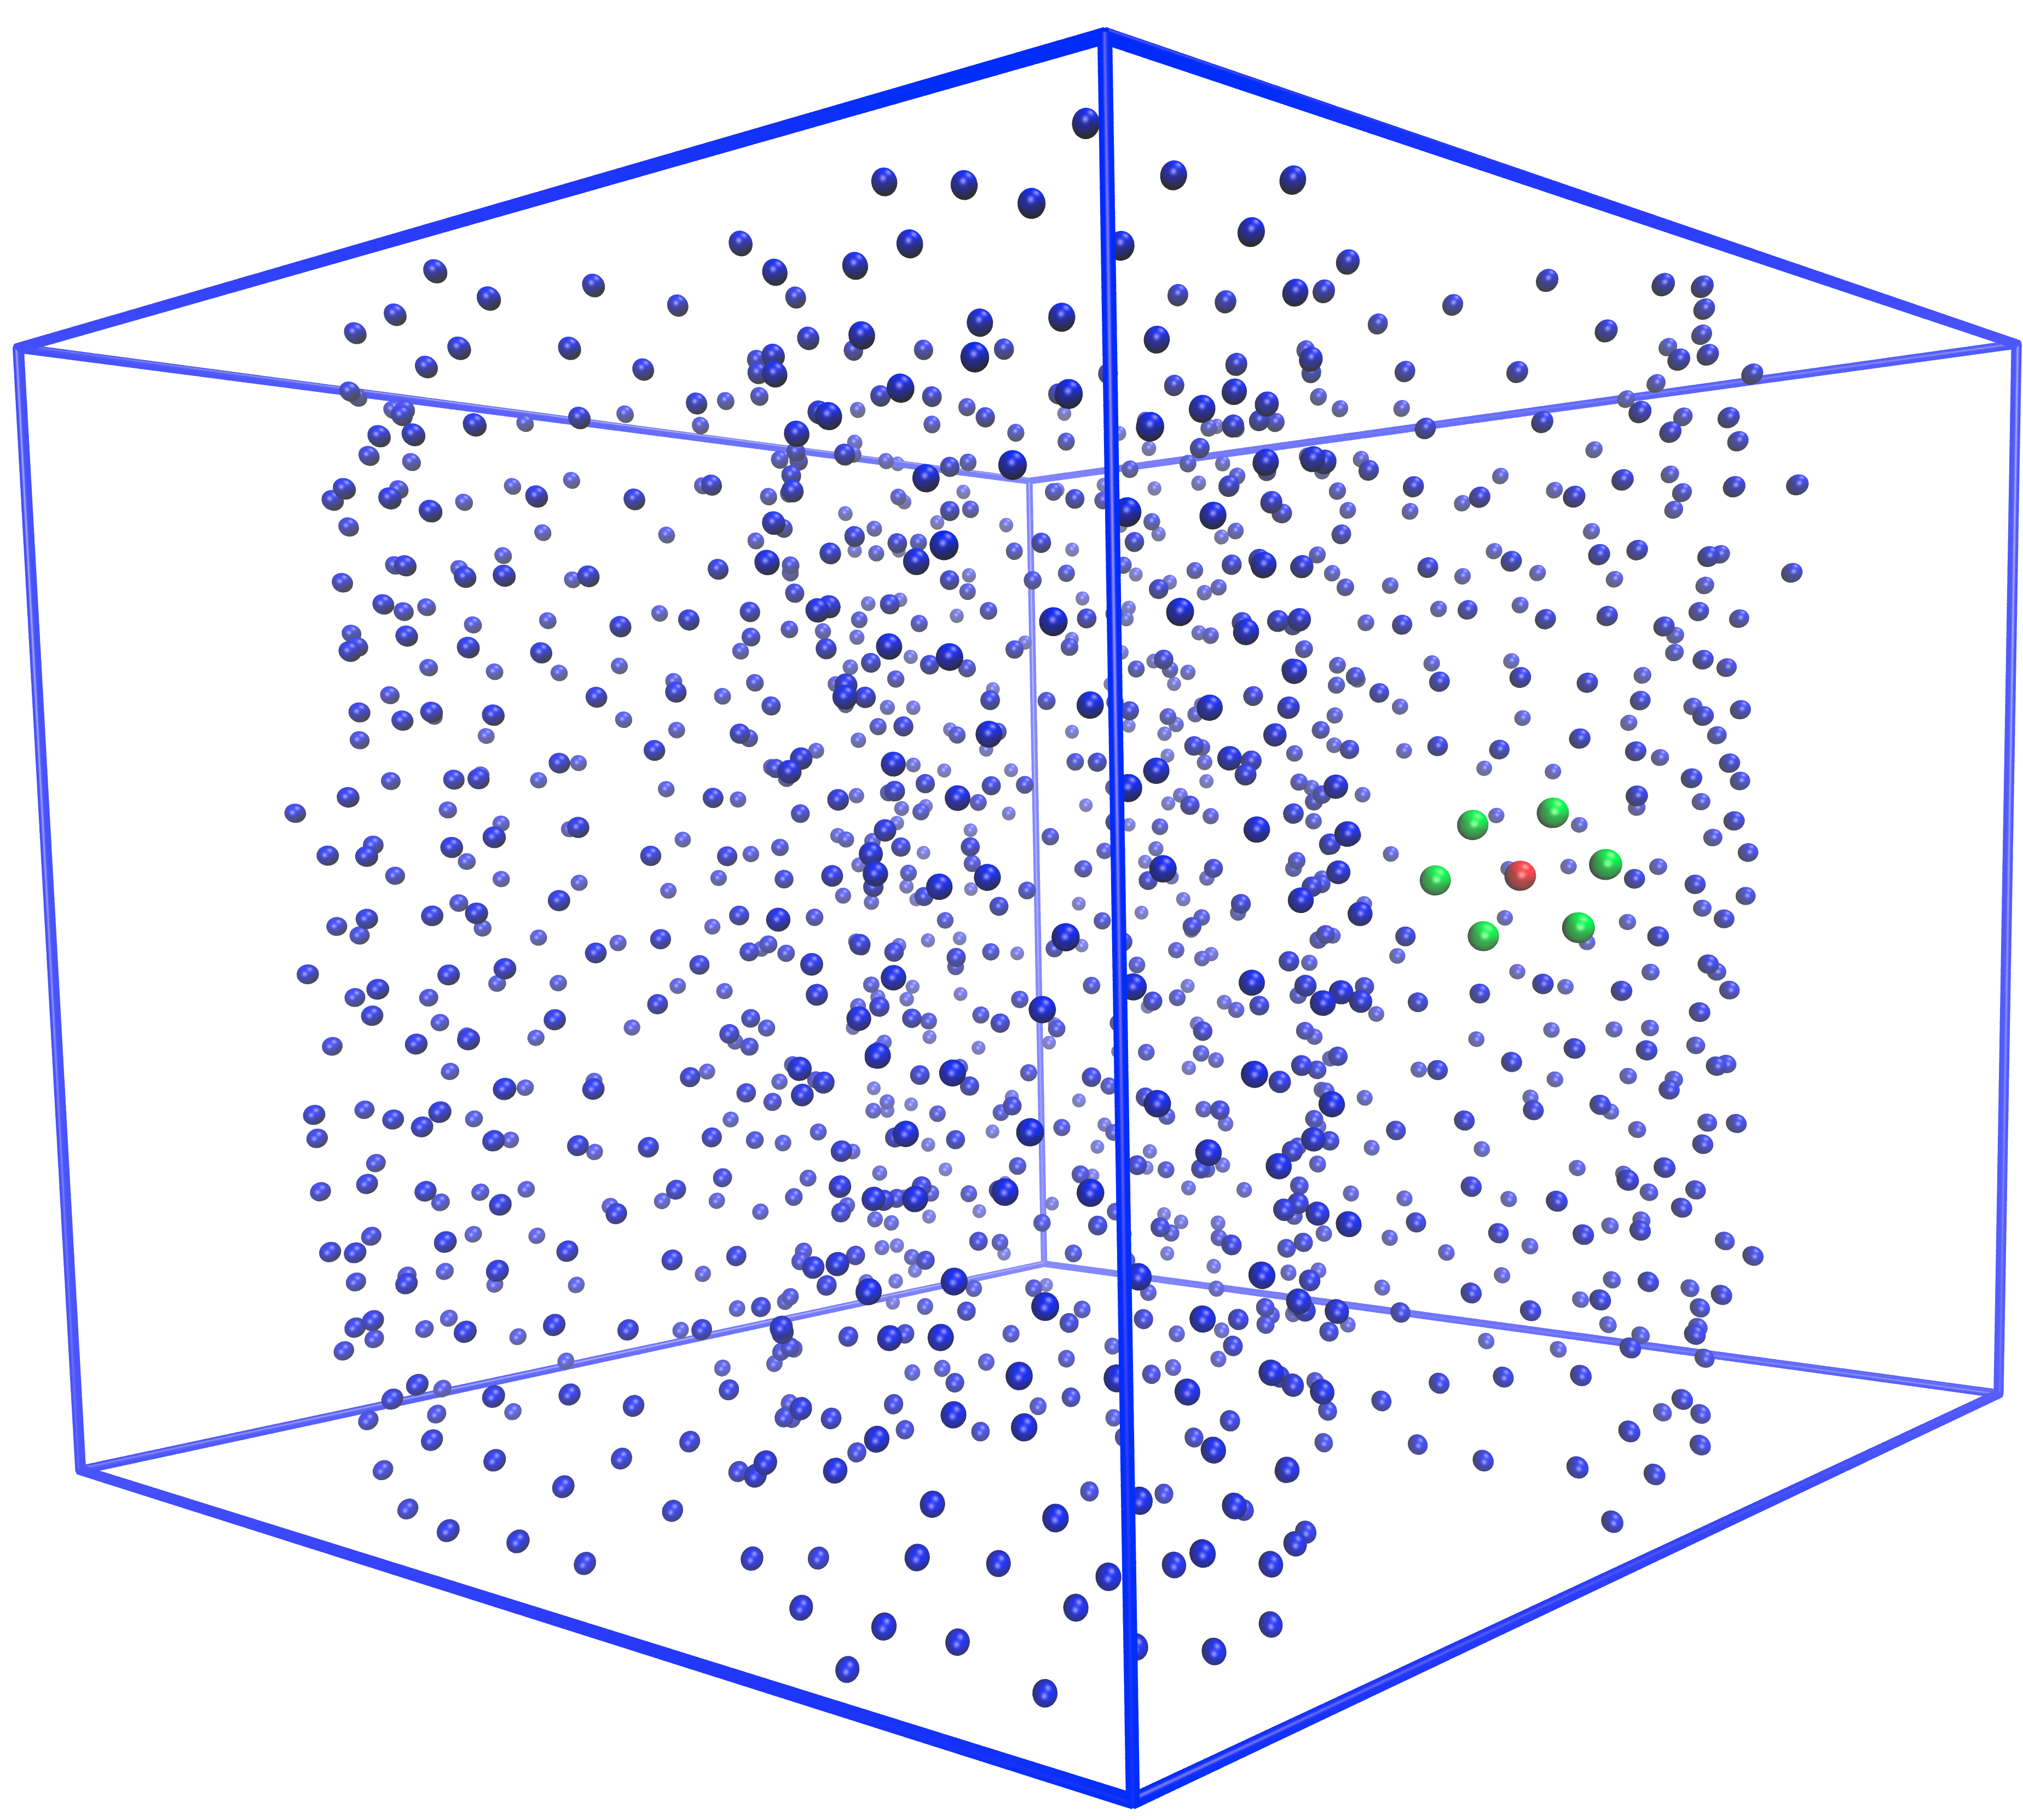
\includegraphics[width=\textwidth]{centroids_box.png}
		\caption{}\label{fig:centroids}
	\end{subfigure}
	\begin{subfigure}{0.45\textwidth}
		\centering
		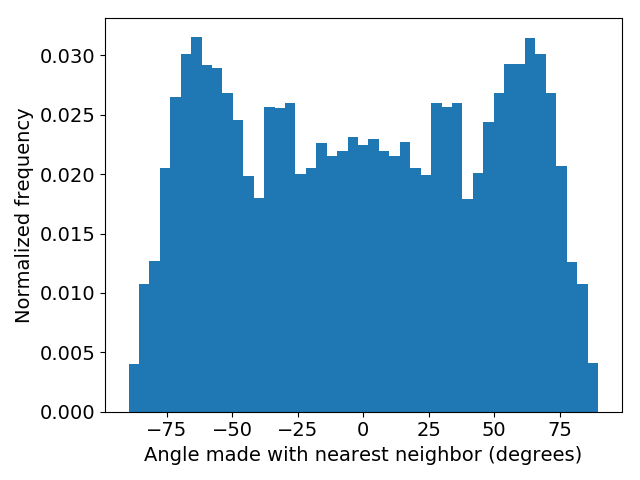
\includegraphics[width=\textwidth]{angles_traj_layered.png}
		\caption{}\label{fig:angle_distribution}
	\end{subfigure}
	\caption{(a) The trajectory can be stripped of all atoms except carbon
	atoms in monomer tails. (b) Simulated diffraction of the tail-only trajectory
	still gives rise to R-spots. (c) Finding the center of mass and visualizing 
	their coordinates reveals the hexagonal-like packing of the tails. (d) The 
	distribution created by measuring the angle between each centroid (e.g. red 
	in (c)) and its neareset neighbors (e.g. green in (c)) with respect to the xy
	plane has distinct spikes near 30\degree, which is consistent with the location
	of R-spots}\label{fig:tail_packing}
  \end{figure}
  %MRS: one could ask the question about basins for the parallel displaced and sandwich as well.  
  %MRS: we had talked a lot about interconversion (or conversion one way but not other?) but 
  %MRS: I think things have changed since then? 
  We can not immediately classify Basin A and Basin B as separate phases.
  \begin{itemize}
	\item To prove the existence of two phases we need evidence of a
	a first order phase transition.
	\item A first order phase transition can be denoted by a discontinuity
        of some order parameter in response to an external condition such as
	temperature.
	\item We chose three easily measurable order parameters: the distance
	between pores, the membrane thickness and the ratio of pore radius to
	the uncertainty in pore radius.  % BJC: these may change
        \item The pore radius is divided by its uncertainty as a way of quantifying
        the degree to which monomers obstruct the pore region.
  \end{itemize}

  Basin B is the dominant configuration at higher temperatures.
  \begin{itemize}
	\item We linearly ramped the temperature of a system in Basin A 
	from 280K to 340K over 100 ns.
        \item Visually, there is a distinct change in pore structure from one
        characteristic of Basin A (Figure~\ref{fig:280K_pore}) to one characteristic of
        Basin B (Figure~\ref{fig:340K_pore}).
        \item The slope of all order parameters changes between 315K and 325K
	(\Cref{fig:p2p_tramp,fig:thickness_tramp,fig:order_tramp}) indicating the
        possibility of an abrupt change in system ordering.
        \item Our 100 ns temperature ramp was likely too fast and caused the system
        to suffer from hysteresis.
  \end{itemize}

  In an attempt to mitigate hysteresis, we performed a slow, stepwise temperature ramp.
  \begin{itemize}
        \item Starting from a sandwiched structure equilibrated at 280K, the system
        temperature was raised to 300K and allowed to equilibrate for 200 ns.
        \item At the end of 200 ns, the temperature was raised 5K and equilibrated
        again for 200 ns.
        \item We continued raising the temperature by 5K and equilibrating for 200 ns
        until the system was equilibrated for 200 ns at 320K.
	\item The same process was repeated with a system equilibrated in Basin B and used
	as a benchmark for comparison. 
  \end{itemize}

  \begin{figure}[!ht]
        \centering
        \begin{subfigure}[b]{0.475\textwidth}
                \centering
                % these next 2 figures are REALLY big (12-18M). Likely could reduce to near 0.5-1.0 MB without loss of 
                % necessary resolution.  A few other figures could have resolution reduced.
                \includegraphics[width=\textwidth]{280K_tramp_close.png}
                \caption{}\label{fig:280K_pore}
        \end{subfigure}
        \begin{subfigure}[b]{0.475\textwidth}
                \centering
                \includegraphics[width=\textwidth]{340K_tramp_close.png}
                \caption{}\label{fig:340K_pore}
        \end{subfigure}
        \vskip\baselineskip
        \begin{subfigure}[b]{0.325\textwidth}
                \centering
                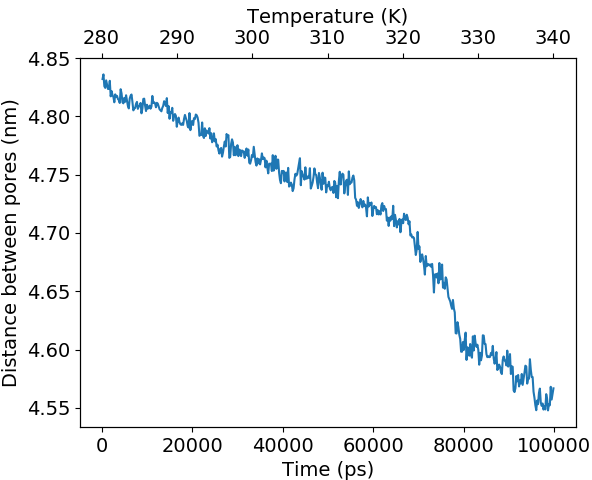
\includegraphics[width=\textwidth]{p2p_tramp.png}
                \caption{}\label{fig:p2p_tramp}
        \end{subfigure}
        \begin{subfigure}[b]{0.325\textwidth}
                \centering
                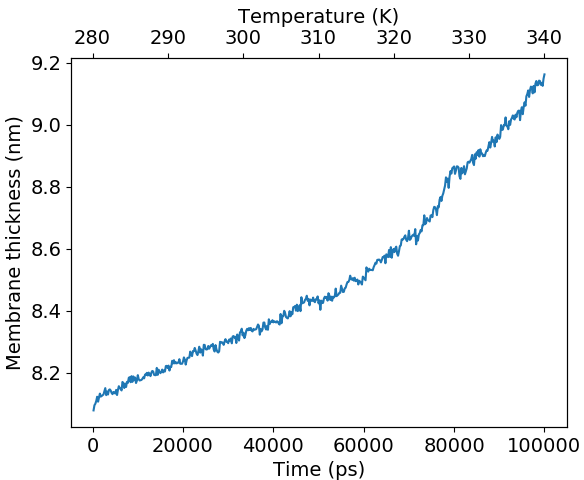
\includegraphics[width=\textwidth]{thickness_tramp.png}

                \caption{}\label{fig:thickness_tramp}
        \end{subfigure}
        \begin{subfigure}[b]{0.325\textwidth}
                \centering
                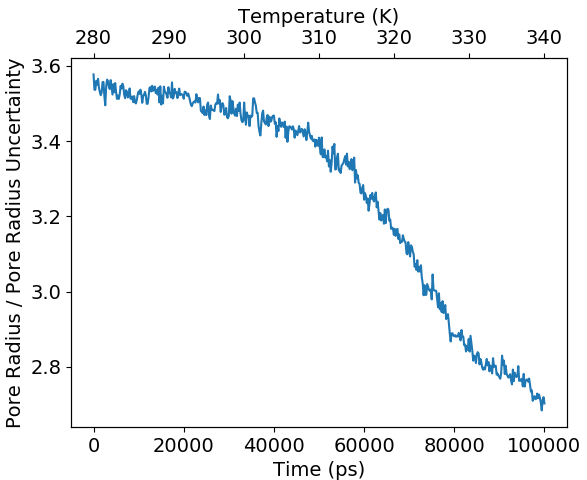
\includegraphics[width=\textwidth]{order_tramp.png}
                \caption{}\label{fig:order_tramp}
        \end{subfigure}
        \caption{(a) The open pore structure exhibited by a structure equilibrated
        at 280K is characteristic of Basin A. (b) The closed pore structure with
        a high degree of radial disorder exhibited when the structure in (a) is
        heated to 340K is characteristic of Basin B. (c) A plot of distance between pores
        vs. temperature changes slope near 325K. (d) A plot of membrane thickness vs.
        temperature changes slope near 325K. (e) The plot of the ratio of pore radius to
        its uncertainty changes slope near 315K.}\label{fig:tramp}
  \end{figure}

  Basin A and Basin B are two configurationally metastable basins.
  \begin{itemize}
        \item There is litle change in disordered phase properties during the 
        temperature ramp.
	\item We observed smooth changes in order parameters as temperature
        of the Basin A system was increased implying that we cannot claim the
	existence of two phases (Figure~\ref{fig:phase_transition}).
	\item Qualitatively, the pore structure of the Basin A system becomes
        comparable to one characteristic of Basin B as temperature is raised. (\Cref{fig:BasinA_280K_pore,fig:BasinB_340K_pore})
	\item The Basin A system does not converge to the same order parameter
	values as Basin B, however it is trending towards Basin B values. (\Cref{fig:p2p_step,fig:thickness_step,fig:order_step})
	\item To resolve the quanitative discrepancy, we would need a slower 
	temperature ramp
	\item Since there are no abrupt changes in any order parameter along the 
	trajectory, we can conclude that the two basins are not separate phases
	\item Basin A is the closest match to what is seen experimentally
	\item Basin B is likely an intermediate between the Col\textsubscript{h} 
	phase and isotropic phase
	\item Basin B is present in our simulations at lower temperatures 
        %MRS: lower temperatures than experiment.  Though nobody has really done the experiments.  
        %MRS: can we conclude anything from some of the in-situ temperature measurements done by Xunda?  We talked about them, but I don't know they are referenced here.
	because our model lacks sufficient pi-pi iteractions necessary to 
	stabilize the system into Basin A. 
  \end{itemize} 

  \begin{figure}[!ht]
        \centering
	% BJC: I'll get actual pictures of the system here. I'm not sure how 
	% necessary this figure is though. It could go in the supplemental 
	% information and I can reference the pictures in the previous figure
	% since they show basically the same idea : Ordered vs. disordered pore
	% Alternatively, I could show two diffraction patterns here from the 
	% beginning and end temperature 
        \begin{subfigure}[b]{0.475\textwidth}
                \centering
                \includegraphics[width=\textwidth]{280K_tramp_close.png}
                \caption{}\label{fig:BasinA_280K_pore}
        \end{subfigure}
        \begin{subfigure}[b]{0.475\textwidth}
                \centering
                \includegraphics[width=\textwidth]{340K_tramp_close.png}
                \caption{}\label{fig:BasinB_340K_pore}
        \end{subfigure}
	\vskip\baselineskip
        \begin{subfigure}[b]{0.325\textwidth}
                \centering
                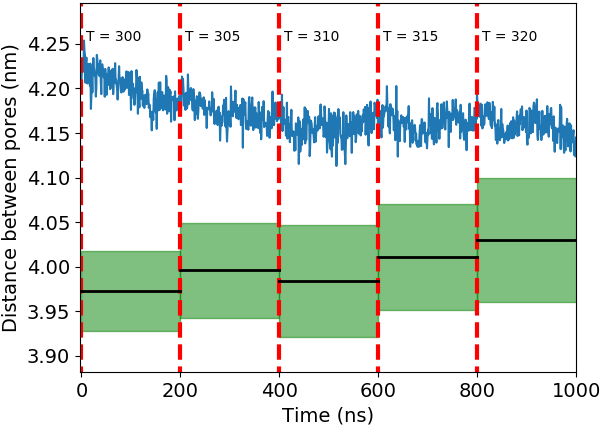
\includegraphics[width=\textwidth]{p2p_layered.png}
                \caption{}\label{fig:p2p_step}
        \end{subfigure}
        \begin{subfigure}[b]{0.325\textwidth}
                \centering
                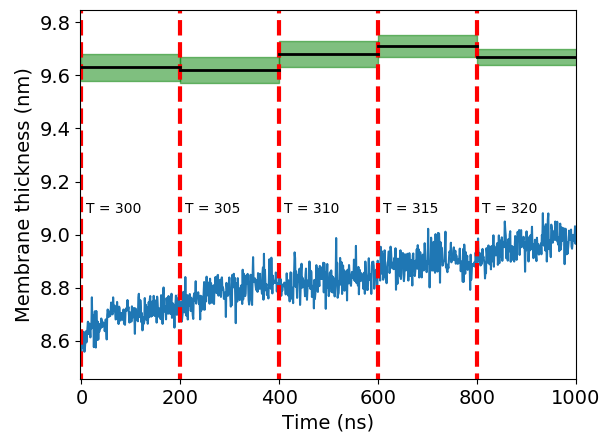
\includegraphics[width=\textwidth]{thickness_layered.png}

                \caption{}\label{fig:thickness_step}
        \end{subfigure}
        \begin{subfigure}[b]{0.325\textwidth}
                \centering
                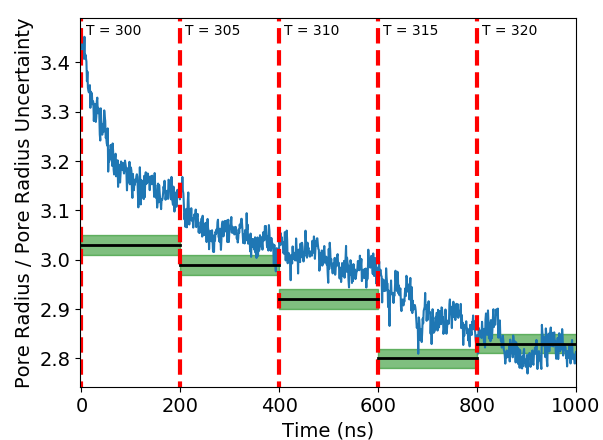
\includegraphics[width=\textwidth]{order_layered.png}
                \caption{}\label{fig:order_step}
        \end{subfigure}
        %MRS: Are (a) and (b) from the nonequilibrium short run?
        %That's not clear. Not clear it's possible to state that it's
        %the ``right'' disordered basin if from the end of a short heating run.

	\caption{In all cases, blue lines represent the measured value of
	the order parameter, black lines are average values calculated from
	equilibrated Basin B systems at each temperature, green shaded regions
	represent the standard deviation of each of the black line values, and 
	red dashed lines show where the temperature is bumped to the next level.
	(a) At 280K, the system is in a configuration reminiscent of
	Basin A. (b) At 335K, the system resembles a Basin B configuration. (c) The pore
	spacing of Basin A decreases with temperature approaching the value 
	exhibited by Basin B. (d) The thickness of Basin A increases smoothly with 
	temperature but is far from the Basin B value. Longer equilibrations at 
	each temperature are needed to allow the system to fully expand. 
        %MRS: might need to explain this ratio better?
        (e) The ratio 
	of pore radius to uncertainty for Basin A changes smoothly with temperature,
	converging to a value below that exhibited by Basin B.}\label{fig:phase_transition}
  \end{figure}

  \subsection*{Ionic conductivity calculation}

  %MRS: which model? Be specific as to which of the above structural ensembles was used.
  The model gives reasonable estimates of ionic conductivity when compared to 
  experiment.
  \begin{itemize}
  	\item Calculated values of ionic conductivity obtained using the Nernst 
	Einstein relation and Collective Diffusion model are compared in 
	Table~\ref{table:conductivity}.
	\item The two methods agree with each other within error, although the 
	uncertainty obtained using the Collective Diffusion model is much higher.
	\item Much longer simulations are needed to lower the uncertainty. % TODO: Run Basin B out longer at same conditions as A
	\item Collective diffusion calculations were generated from 
	500 ns simulations.
	\item Our calculated values would benefit from longer simulations. 
	\item For this reason we will likely only use the Nernst Einstein relation
	in future calculations of this type. 
	\item Interestingly, Basin B has a higher ionic conductivity than Basin A.
	\item We hypothesize that conductivity is enhanced in Basin B due to a 
	higher sodium ion diffusivity.
	\item Transport of sodium is likely facilitated by the homogeneity of Basin B.
	Sodium ions have less sites to move to in Basin A.
        % total number of sites is the same in both basins, correct? -- do you mean that in basin B, there are more nearby sites?
	\item There is currently no experimental evidence of this trend. Maybe Xund will find something
	\item In both cases, our calculated values for Basin A are higher than the 
	experimental values, as expected. 
	\item Some of the discrepancy is likely a result of using an imperfect forcefield. 
	\item However, the real system, although mostly aligned and straight, has a 
	distribution of azimuthal angles, meaning that the pores have a degree of 
	tortuosity which lowers the effective ionic conductivity of the bulk membrane. 
	\item The ordering from isotropic to mostly aligned mesophases showed an 85 
	fold increase in ionic conductivity. We would expect additional gains in a 
	perfectly aligned system.
  \end{itemize}
	
  \begin{table}[h]
  \centering
  \begin{tabular}{ccc}
  \toprule
  \multicolumn{3}{c}{Calculated Ionic Conductivity \si{\siemens\per\meter}} \\
  \hline
  Method & Basin A & Basin B \\
  \midrule
  Nernst Einstein & \num{1.23e-4} (0.01) & \num{1.76e-4} (0.02) \\
  Collective Diffusion & \num{1.40e-4} (0.32) & \num{4.6e-4}(2.4) \\
  Experiment & \num{1.33e-5} (0.10) & -- \\
  \bottomrule
  \end{tabular}
  \caption{Calculated ionic conductivity using Nernst-Einsten and Collective Diffusion 
  agree within error. Both methods give calculated values of ionic conductivity which
  are an order of magnitude higher than experimental values~\label{table:conductivity}}.
  \end{table}

  %MRS: the next sections maybe should be supporting?
  %MRS: you say ``the distance decreases by 1 A'' but is that true
  %over all of the different structures? 
  %MRS: Maybe show the difference before and after crosslinking in X-ray, to show that you can't tell?
  %MRS: you don't otherwise discuss clearly what effect crosslinking would have. 
  \subsection*{Implementation of the crosslinking algorithm}

  We applied the crosslinking algorithm to the equilibrated sandwiched structure in 
  Basin A.
  \begin{itemize}  %BJC: working on the following. The following is what I expect
  	\item There is an even distribution of crosslinks between same monomer tails, 
	between monomers in the same pore and between monomers in different pores 
	including periodic boundaries.
	\item The distance between pores shrinks by 1 \angstrom after the system is 
	crosslinked
	\item Major features are still present in the X-ray diffraction
	\item The ionic conductivity is higher/lower in the crosslinked system
  \end{itemize}
  %BJC: THe following figure will be replaced with one representative of the new
  % data I am  collecting above.
  \begin{figure}[!ht]
	\centering
	\begin{subfigure}{0.31\textwidth}
		\centering
		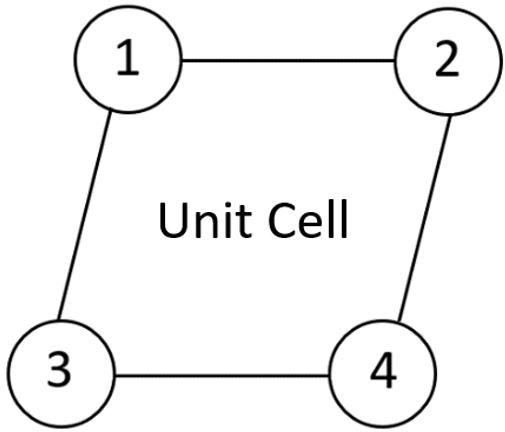
\includegraphics[width=\textwidth]{p2p_diagram.PNG}
		\caption{}\label{fig:p2p_diagram}
	\end{subfigure}
		\begin{subfigure}{0.31\textwidth}
		\centering
		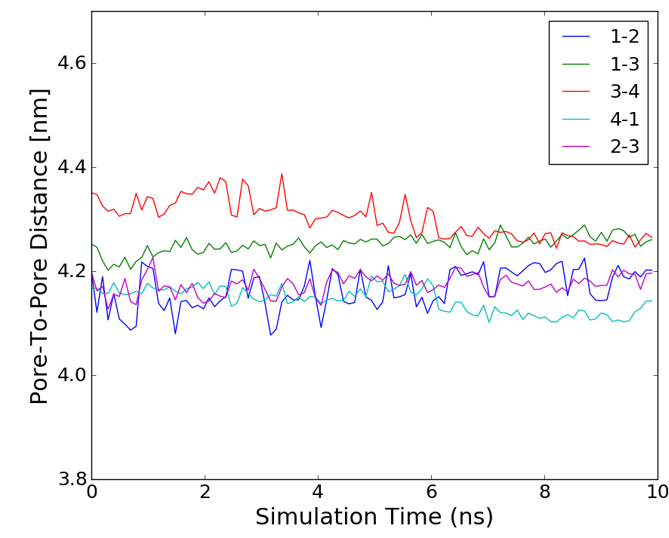
\includegraphics[width=\textwidth]{no_xlink_p2p.png}
		\caption{}\label{fig:no_xlink_p2p}
	\end{subfigure}
		\begin{subfigure}{0.31\textwidth}
		\centering
		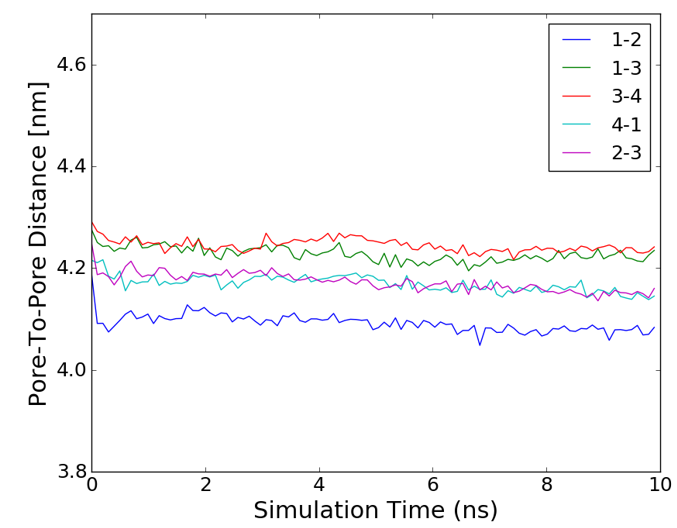
\includegraphics[width=\textwidth]{xlink_p2p.png}
		\caption{}\label{fig:xlink_p2p}
	\end{subfigure}
	\caption{(a) The legends of the plots in (b) and (c) refer to the numbers shown.
	Each numbered circle represents a pore. Distances are measured along each of the 
	lines shown in addition to the distance from pore 1 to pore 4. (b) The positions
	of individual pores fluctuate in an uncrosslinked system. (c) The positions of
	individual pores in the crosslinked system are stable relative to the uncrosslinked
	system}\label{fig:xlink}
  \end{figure}

\clearpage
\bibliography{llc}

\end{document}
